\chapter{数据驱动的着色器程序性能预测方法}

\label{sec:begin_of_ch3}

根据对前面相关工作的调研和分析,本章将提出一种数据驱动的着色器程序性能预测方法。该方法利用 Transformer 模型,从实际测量的性能数据中学习各个架构的性能特点,而无需逐平台设计基于分析的性能模型。

为了构造一个与平台独立的预测方法,本方法选择只依赖于应用程序呈递到图形 API 的信息。SPIR-V \cite{SPIRV} 是 Vulkan 中着色器程序使用的中间表示格式,而本研究选择基于 SPIR-V 构建预测器的原因有三:第一,有相关工作 \cite{pmlr-v139-peng21b, Niu2023fair} 提到中间表示是一种将程序的特点暴露给基于学习的模型的好的选择;第二,为了保证本章提出的方法平台独立,输入的格式必须和真正被 GPU 执行的、经常缺乏文档的设备原生指令结构解耦;第三,由 Khronos Group 和相关厂商打造的 SPIR-V 生态系统提供了很多用于程序变换、优化和模糊测试的软件工具,可以对本方法的构建起到一定帮助。

一般来说,一条特定指令的执行时间不仅与其执行的操作有关,还与其上下文信息有关。对于 GPU 原生指令,执行时间受到其执行的操作、操作数的数据类型、操作数的可用性以及后端算术逻辑单元的占用率的影响。此外,对于 SPIR-V IR 指令来说,其还将经历一系列与局部和全局上下文信息相关的转换,以降级(lowering)到 GPU 原生指令。这些依赖于上下文的行为,在 SPIR-V 层次上即表现为指令的执行时间会受到其所在指令序列中其它指令和其排列顺序的影响。因此,此问题可以被建模为一个序列学习问题,并可以应用 Transformer\cite{Vaswani2017AttentionIA} 来作为预测器的网络架构。

尽管着色器本身是用一种 DSL 来编写的,但在现代硬件上执行的着色器可以包含动态的循环和分支指令,从而使着色器程序语言在理论上即具有图灵完备性。在图灵完备计算模型内,用户有能力构建无法判定的停机问题\cite{10.1112/plms/s2-42.1.230},这说明仅靠着色器程序输入和程序表示本身来预测其性能在理论上是不可解的。因此,为了准确预测着色器行为,预测器框架有必要提供额外的信息来处理这种理论上即可分析出的局限性。同时可以注意到,管线后期的着色器程序的调用计数由三角形输入、先前的管线阶段和 Uniform 输入决定,而不同的计数会显著影响总执行时间。基于这些观察,本方法选择在 IR 的层次上进行着色器指令跟踪,从而为随后构造的预测模型提供额外的信息以供学习。应该注意的是,本文提出的跟踪阶段可以在任何其他能够运行待测试着色器的平台上完成,从而保持预测器的平台独立性。

\section{方法总览}

\begin{figure}[h]
  \centering
  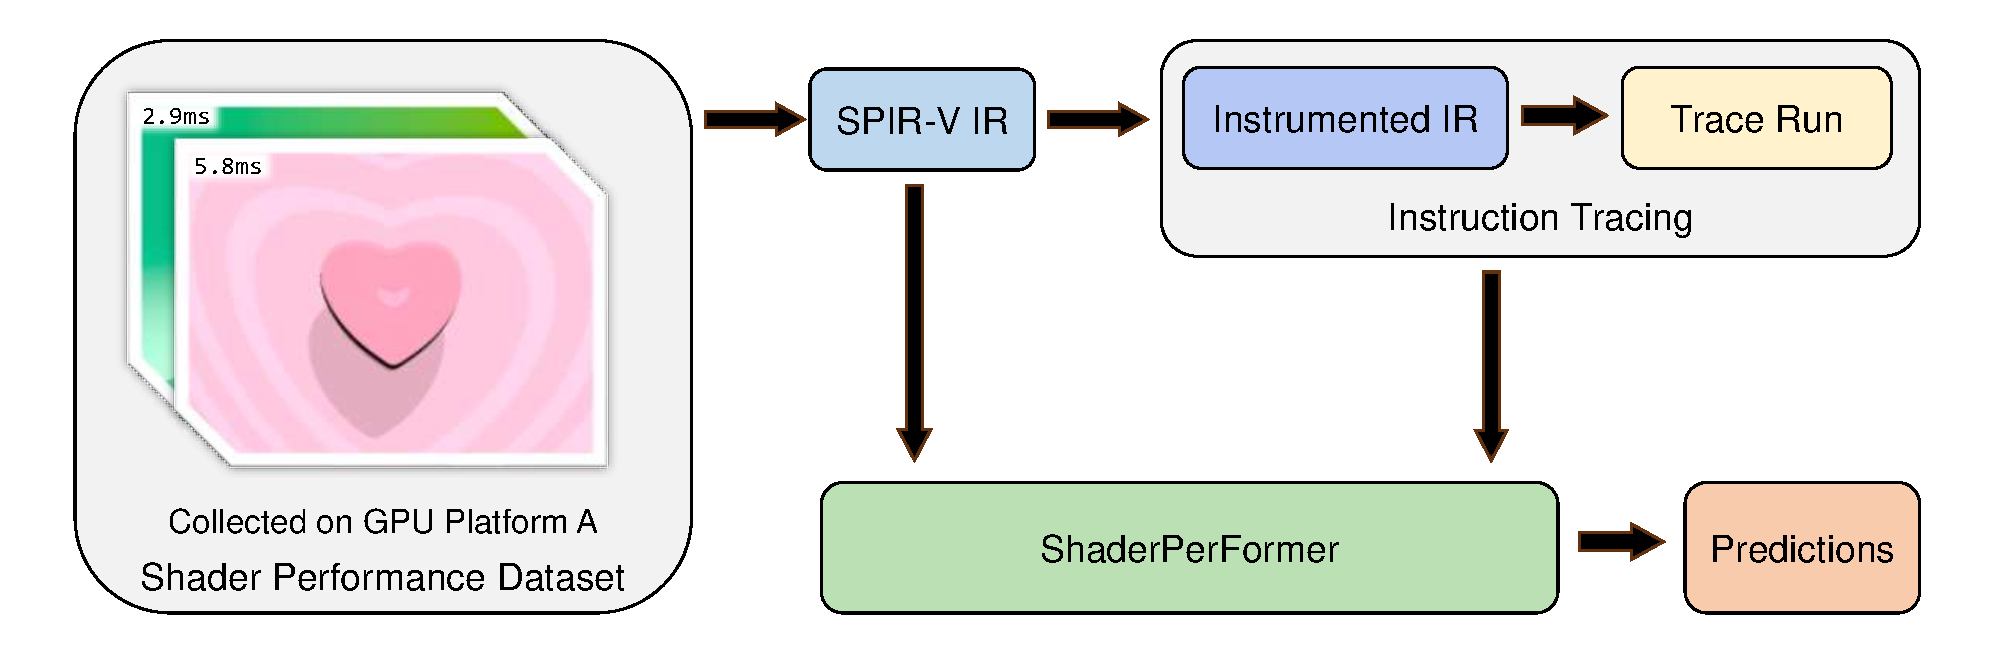
\includegraphics[width=1\linewidth]{figures/OverviewNewNewNew.pdf}
  \caption{本研究提出的方法总览}
  % \note{注:图中 GPU 平台 A 是待建模的 GPU 平台,本文提出的模型使用 GPU 平台 A 上收集到的性能数据进行训练。}
  \label{fig:pipeline_overview}
\end{figure}


本研究提出的方法构建了一个针对特定图形处理平台的着色器性能预测模型。该方法可以分为几个主要步骤:着色器数据集构造,着色器指令追踪,以及利用模型进行性能预测。这些环节的大致流程如图 \ref{fig:pipeline_overview} 所示。

首先,为了预测目标图形处理器平台的着色器性能,本研究提出的方法需要收集一个详尽的着色器性能数据集,该数据集收集过程的具体讨论可以参见第 \ref{sec:dataset} 节。该数据集不仅包含丰富的着色器 GLSL 源代码、编译后的 SPIR-V 中间表示,还包括每次着色器在目标平台运行时着色器的 Uniform 输入参数,以及这些着色器在目标 GPU 平台运行测得的执行时间。这些数据是本方法所述预测器学习理解着色器性能的“原材料”,也为后续的模型训练和验证提供了比较扎实的基础。

数据收集完成后,本研究提出了一个基于学习的、能够准确预测着色器在目标 GPU 平台上执行时间的模型 ShaderPerFormer。为了达成这个目标,该模型需要两类输入:一是以 SPIR-V 中间表示格式来进行表示的着色器指令;二是该着色器的指令执行跟踪信息。

原始指令的收集,是通过使用业界标准的着色器编译器 glslang \cite{glslang} 实现的,而着色器执行跟踪信息则是通过一个专门的指令跟踪阶段(见第 \ref{sec:tracing} 节)来获取的。在指令跟踪阶段,本研究提出的过程会对着色器原始的 SPIR-V 中间表示插入额外的跟踪指令,然后运行修改后的中间表示,来统计出执行过程中 SPIR-V 粒度的指令运行计数。这些带有跟踪指令的 SPIR-V 中间表示可以在目标平台运行,也可以在其它非目标平台运行。通过着色器指令跟踪过程,本研究提出的方法能够较为准确地追踪和分析着色器的执行行为,而无需再在目标平台上实际的执行着色器程序。

随后,本研究提出的方法将收集到的 SPIR-V 指令和着色器执行跟踪信息一同,输入到构建的神经网络模型 ShaderPerFormer (见第 \ref{sec:model} 节)中。该模型将根据这些输入进行推理,得到对绘制一帧所需的时间的预测。进而,本研究利用数据集中的测量的真实值来计算损失函数的损失值,并用梯度下降的办法对模型进行优化。


\section{着色器程序性能数据集}

\label{sec:dataset}

为了学习着色器程序的性能,预测器的构造首先需要丰富的着色器程序。针对这一点,本方法选择利用 Shadertoy \cite{Shadertoy} 平台上用户上传的着色器资源。

Shadertoy 是一个在线平台,它允许用户创建、分享和查看着色器程序及其渲染的结果。基于光栅化的图形渲染程序通常需要指定管线的顶点和三角面索引输入,同时给出过程中用到的顶点、片元等着色器。不过,为了降低上手门槛,让用户的精力专注于创造新奇有趣的视觉效果本身,Shadertoy 平台上的着色器均有一个“直通”的顶点着色器(亦即,顶点在顶点着色器定义的顶点变换阶段均按原样输出),且输入图元为覆盖全视口的两个三角形。

例如,一个简单的 Shadertoy 着色器可能如图 \ref{fig:example_glsl_shadertoy_code} 中的代码所示,而其输出类似图 \ref{fig:example_shadertoy_output} 所示。可以看到在 Shadertoy 中,简单的代码就可以创造丰富的效果。

\begin{figure}  % 'h' for here, 't' for top, 'b' for bottom, 'p' for on a separate page
\centering

\begin{lstlisting}[language=GLSL]
void mainImage( out vec4 fragColor, in vec2 fragCoord )
{
    // 从 0 到 1 的归一化屏幕坐标
    vec2 uv = fragCoord/iResolution.xy;

    // 生成随时间 iTime 变化的像素颜色
    vec3 col = 0.5 + 0.5*cos(iTime+uv.xyx+vec3(0,1,5));

    // 输出到屏幕
    fragColor = vec4(col,1.0);
}
\end{lstlisting}
\caption{在屏幕上产生渐变颜色的 Shadertoy 代码示例}
\label{fig:example_glsl_shadertoy_code}
\end{figure}

\begin{figure}
\centering

\includegraphics[width=0.7\textwidth]{figures/example_shadertoy_output.png}
\caption{在屏幕上产生渐变颜色的 Shadertoy 效果示例}
\label{fig:example_shadertoy_output}
\end{figure}

尽管在渲染时缺乏多样的几何输入,在 Shadertoy 上进行开发的用户仍然可以通过应用如光线步进(Ray Marching)\cite{Hart1996}, 过程化内容生成(Procedural Content Generation)等技术来创建能够产生复杂视觉效果的着色器。图 \ref{fig:shadertoy_gallery} 展示了一些 Shadertoy 中着色器的渲染结果和其主要采用的渲染技术。

\begin{figure}[htbp]
    \centering
    \begin{minipage}[b]{\textwidth}
        \begin{subfigure}[b]{0.48\textwidth}
            
\includegraphics[width=\textwidth]{figures/shadertoy_cloud.png}
            \caption{过程化纹理生成 (PTG)}
            \label{fig:sub_textgen}
        \end{subfigure}
        \hfill % Adds horizontal space between the subfigures
        \begin{subfigure}[b]{0.48\textwidth}
            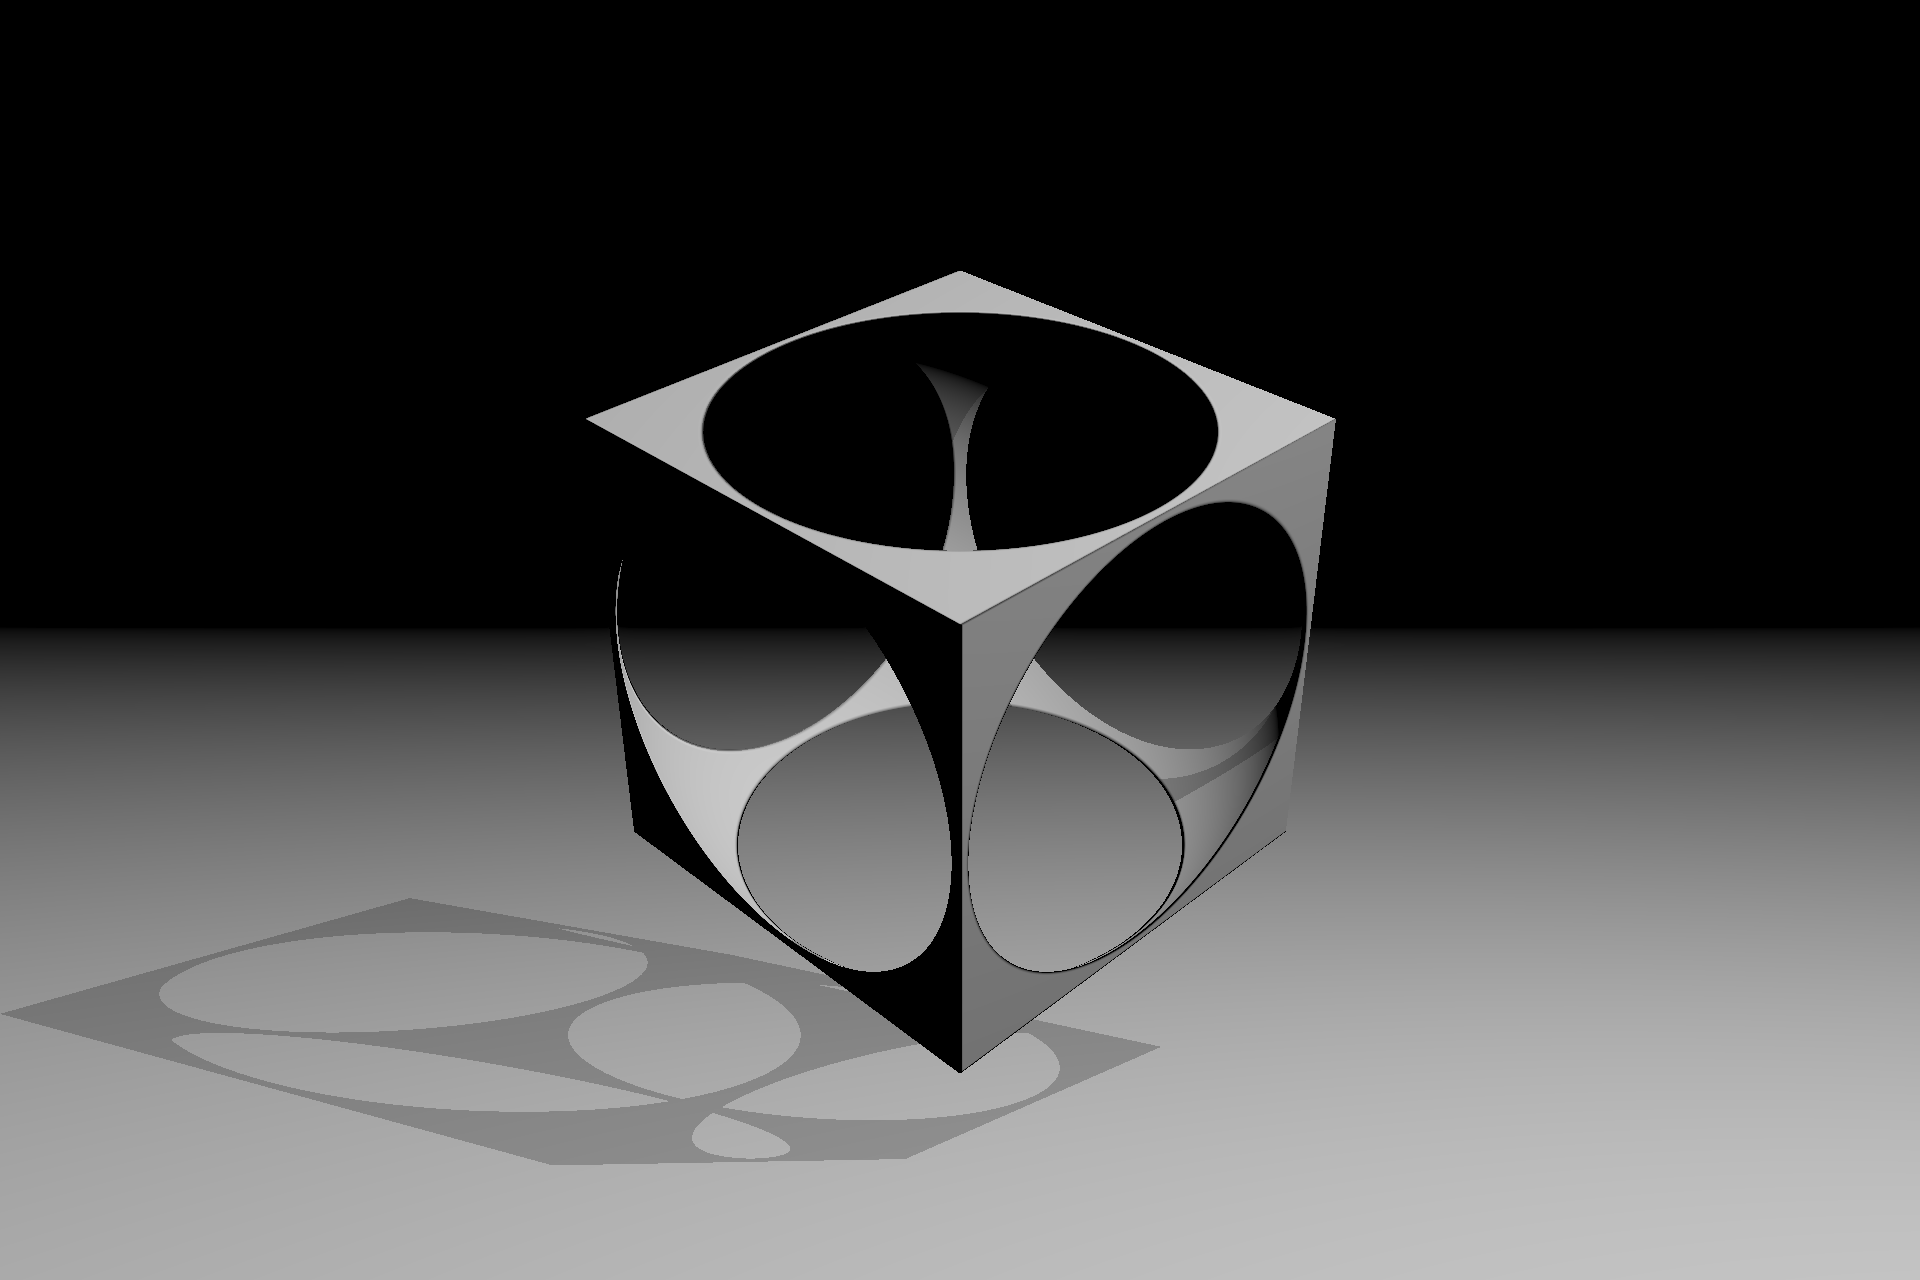
\includegraphics[width=\textwidth]{figures/shadertoy_csg.png}
            \caption{构造实体几何 (CSG)}
            \label{fig:sub_csg}
        \end{subfigure}
    \end{minipage}
    
    %\vspace{1em} % Adds vertical space between the rows of subfigures
    
    \begin{minipage}[b]{\textwidth}
        \begin{subfigure}[b]{0.48\textwidth}
            
\includegraphics[width=\textwidth]{figures/shadertoy_raymarching.png}
            \caption{光线步进 (Ray Marching)}
            \label{fig:sub_raymarching}
        \end{subfigure}
        \hfill % Adds horizontal space between the subfigures
        \begin{subfigure}[b]{0.48\textwidth}
            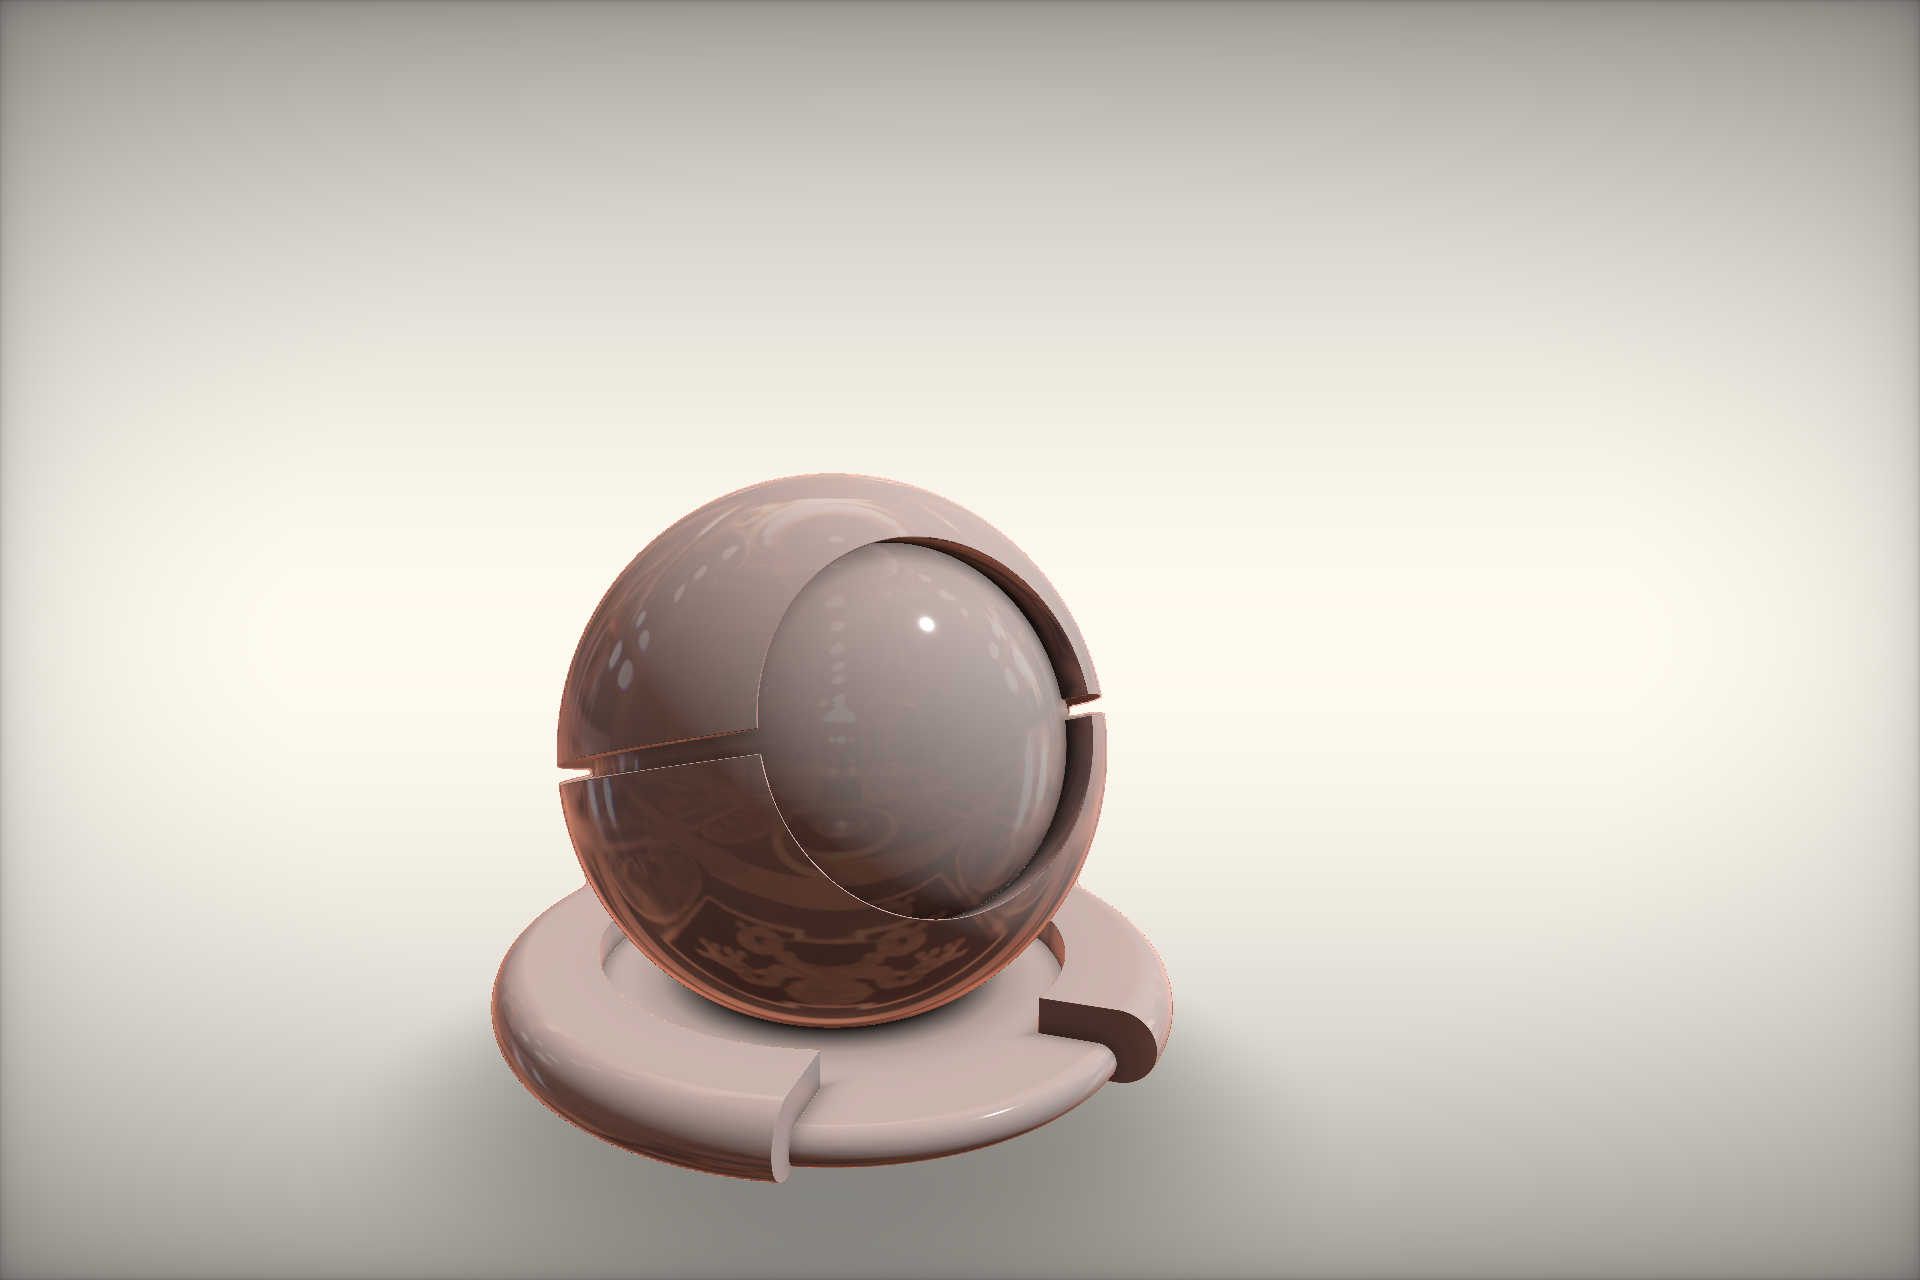
\includegraphics[width=\textwidth]{figures/shadertoy_pbr.png}
            \caption{基于物理的着色 (PBS)}
            \label{fig:sub_pbs}
        \end{subfigure}
    \end{minipage}
    
    \caption{Shadertoy 用户\cite{ShdrToyUser1, ShdrToyUser2}着色器程序效果示例与其使用的主要技术}
    \label{fig:shadertoy_gallery}
\end{figure}

Shadertoy 网站收集的着色器在渲染技术方面覆盖相当完备,故而笔者认为 Shadertoy 上的着色器在片元着色器性能建模方面具有代表性。下面,本文将依次阐述数据集构造的主要步骤。

\subsection{数据收集}

为了方便第三方程序的编写,Shadertoy 网站提供了基于 HTTP GET 的 API 接口,这为本研究的数据收集工作提供了一定便利。利用 Shadertoy API 进行数据收集的步骤大概如下:

\begin{enumerate}
    \item 在 Shadertoy 网站上申请 API Key,从而得到 6 位的 API Key
    \item 请求 \url{https://www.shadertoy.com/api/v1/shaders?key=APIKey},以得到所有用户上传的着色器的 ID
    \item 对每个 ID,请求 \url{https://www.shadertoy.com/api/v1/shaders/shaderID?key=AppKey} 以得到 JSON 格式存储的着色器
\end{enumerate}

之后,需要将 Shadertoy 输出的 JSON 文件筛选,并处理成预测器需要的 glslang 可编译的单文件 GLSL 格式。为此,本文将简单介绍一下 Shadertoy 的 JSON 的文件模式。

Shadertoy 的 JSON 文件中描述了该着色器上传的用户、描述、修改时间等一些元信息,以及该着色器拥有的所有渲染通道(Render Pass)信息。在这里,一个渲染通道内包含的信息大致对应着一次图形流水线绘制需要的纹理、Uniform 变量输入和着色器程序资源,且不同的渲染通道之间对应的图形流水线绘制具有固定的先后顺序。Image 通道负责最后的画面输出,其是必须存在的,其它通道则通常作为 Image 通道的输入,为可选的。下面是常见的渲染通道的简单介绍:

\begin{enumerate}
    \item Image 通道:这是渲染通道的基础部分,用于生成每一帧最后显示的图像。在这个通道中,可以定义和操作像素颜色、纹理坐标和其他与图像生成相关的功能。
    \item Common 通道:Common 通道不是一个真正的渲染通道,而是被作为着色器程序的一部分,以字符串的形式插入到每个其他渲染通道的着色器当中。故而,该通道一般用于定义在可以在整个着色器程序中重复使用的,多个渲染通道中共享的函数例程。
    \item Buffer 通道:Buffer 通道用于存储和操作着色器程序的一些中间数据。这些通道可以用于记录程序状态或者进行一些复杂图像效果的构建。每个 Buffer 通道的绘制会绘制到专门的图像缓冲区中。
\end{enumerate}

对于 Shadertoy 的着色器程序来说,可以认为使用了 Buffer 通道的程序为多渲染通道程序,而只使用 Image 和 Common 通道的程序为单渲染通道程序。由于多渲染通道的程序可以认为是多个独立的单渲染通道程序的叠加,故而本研究在构建数据集时只着眼于处理单渲染通道的着色器程序。

\subsection{后处理和编译}

Shadertoy 上的着色器程序运行时需要在每帧提供一些预先设置好的 Uniform 变量资源。这些 Uniform 变量作为输入,其本身可以以 GLSL 的匿名 Uniform 块的形式被源码所引用,且可以大致分为屏幕数据、用户输入、时间和其它通道输入采样四种类别。例如,图 \ref{fig:example_glsl_shadertoy_code} 就使用了 iResolution 和 iTime 两个 Uniform 变量。一些常用的 Uniform 输入包括:
\begin{itemize}
    \item iTime: 当前的渲染时间
    \item iFrame: 当前渲染的帧编号
    \item iResolution: 当前的屏幕分辨率
    \item iMouse: 鼠标位置
    \item iDate: 年月日和时间信息
\end{itemize}

许多 Shadertoy 程序对上述输入进行更改的情况下,会产生出不同的画面。同时,Shadertoy 着色器程序的入口点函数 mainImage 与通常的片元着色器入口点函数不同。在 Shadertoy 网站上,用户上传的编译器会被拼接为 WebGL 可以执行的 OpenGL ES 着色器程序,并由浏览器的 WebGL 实现运行。

类似的,本方法首先用文本处理的办法在程序源文件前补充相应 Uniform 变量的定义和用于调用真正入口点 mainImage 的片元着色器 main 函数,随后使用 glslang 编译器将这些着色器编译为适用于 Vulkan 的 SPIR-V 中间表示。对于图 \ref{fig:example_glsl_shadertoy_code} 中的示例着色器程序补全后的代码大致如图 \ref{fig:example_glsl_composed_code} 所示。

\begin{figure}  % 'h' for here, 't' for top, 'b' for bottom, 'p' for on a separate page
\centering

\begin{lstlisting}[language=GLSL]
#version 310 es
precision highp float;
precision highp int;
precision mediump sampler3D;

// 设置好正确的颜色输出变量布局
layout(location = 0) out vec4 outColor;

layout (binding=0) uniform PrimaryUBO {
  uniform vec3 iResolution;
  uniform float iTime;
  // ...省略了一些 Uniform 变量
};

void mainImage(out vec4 c, in vec2 f);

// 插入并调用真正的 main 函数
void main() {mainImage(outColor, gl_FragCoord.xy);}

// 下面粘贴原 Shadertoy 代码
void mainImage( out vec4 fragColor, in vec2 fragCoord )
{
    vec2 uv = fragCoord/iResolution.xy;
    vec3 col = 0.5 + 0.5*cos(iTime+uv.xyx+vec3(0,1,5));
    fragColor = vec4(col,1.0);
}
\end{lstlisting}
\caption{在屏幕上产生渐变颜色的 Shadertoy 代码示例}
\label{fig:example_glsl_composed_code}
\end{figure}

\subsection{性能测量}
\label{sec:perf_measure}

Shadertoy 着色器在 Shadertoy 运行时使用了 WebGL 作为运行时环境,而 WebGL 根据浏览器环境的不同,又可被 ANGLE 等浏览器中的中间件转译为 Vulkan, OpenGL ES, OpenGL 和 Direct3D 等调用。相对冗长的调用链路,让使用浏览器直接对性能进行测量带来了一些麻烦。

为了得到比较精确的测量结果,本研究选择使用一个独立的 Vulkan 程序来运行着色器,并且用 Vulkan 的时间戳计数器读取 (timestamp counter query)功能来进行较为精确的 GPU 时间测量。同时,为了方便和预测器进行交互,以及实现各种不同的计时模式、运行参数的控制,这里选择将此 Vulkan 程序利用 pybind11 函数库封装为一个 Python 扩展,并在扩展中操作 Vulkan 上下文。这个名为 vkExecute 的扩展可以比较方便的和其它用 Python 写的数据集管理模块、实验计划运行模块,以及后面用 PyTorch 写就的预测模块比较好的结合。

该 Python 扩展的核心的性能测量逻辑可以参考算法 ~\ref{alg:profile}。为了减少 CPU 提交时的额外开销对性能数据的影响,本方法采用基于 GPU 的时间戳计数器来精确测量执行时间。这其中的 unitTs 表示计数器每次增加所对应的时间间隔,这一值依赖于具体的硬件平台。由于许多收集到的着色器在现代 GPU 平台上的执行速度非常快(典型值大于 1000 fps),所以为了进一步降低 GPU 绘制流水线启动的额外开销对测量值的影响,本方法在时间戳计数器读取之间共发出 num\_cycles 次绘制命令。此外,为了确保结果的准确性,本方法会进行 num\_trials 次 GPU 命令提交,并将每次提交前后的 GPU 时间戳相减,再乘以 unitTs,以得到每次 GPU 命令执行所消耗的时间。所有的测量结果都会存储以供后续分析。

同时,为了确保结果的稳定性,在实验运行时笔者通过各个 GPU 厂商提供的命令行工具,在测试过程中锁定了待测试 GPU 的着色器和内存时钟频率,并在测量过程中多次监测,以确保没有因为 GPU 自身的自动功耗控制机制影响测量结果。

\subsection{错误恢复}

\label{sec:error_recovery_and_filters}

由于 Shadertoy 平台并不对用户提交的着色器进行合法性验证,因此对于某些用户提交的着色器,编译错误可能发生。同时,由于着色器语言本身的图灵完备性,其执行时间可能没有上限,这可能导致现代 GPU 驱动程序在渲染命令耗时过长时触发引擎或 GPU 的重置\cite{TDRWindows}。当此类重置事件发生时,性能测量例程的 Vulkan 上下文会失效。为了避免整个程序被意外终止,本研究提出的 Python 扩展 vkExecute 会将着色器性能测量的任务放到独立的子进程中运行,并在运行完成后在数据库中原子更新本次测量的结果。

同时,我们在导出数据时会额外进行一些数据的筛选,以确保测量数据的正确性。这些筛选主要包括以下几类过滤:
\begin{itemize}
    \item 单渲染通道过滤:过滤出只有 Image 和 Common 渲染通道的着色器。
    \item 运行和追踪成功过滤:过滤出运行和 SPIR-V 指令追踪阶段成功的性能样本。
    \item 非纯黑纯白过滤:将运行得到的图像与纯黑、纯白图像进行比较,如果相同则排除该性能样本,以比较保守的过滤因为驱动实现不同产生的渲染 bug 等情形。
    \item 词元长度限制过滤:计算着色器 SPIR-V 表示在通过分词器分词后的长度,过滤因为过长导致送入网络进行训练和预测较为困难的着色器。
    \item 时间限制过滤:部分着色器的测量结果为异常大的值,这些通常是着色器运行时间过长,而因为驱动 bug 导致的边界情况,应当予以过滤。
\end{itemize}

其中时间限制过滤使用 10 秒,词元长度限制选择为 4096 个词元。表 \ref{table:datasetFilters} 给出了实际测量时经过过滤器过滤后的性能样本数量一览。

\begin{algorithm}
\caption{性能测量例程伪代码}
\label{alg:profile}

\SetAlgoLined % For setting line numbering
\SetKwFunction{FProfileShaderOnce}{ProfileShaderOnce}
\SetKwFunction{FProfileShader}{ProfileShader}
\SetKwProg{Fn}{Function}{:}{}
\SetKwArray{VecResults}{results}

\Fn{\FProfileShaderOnce{num\_cycles}}{
    执行图像内存屏障、布局转换并重置时间戳查询池\;
    等待先前命令完成\;
    cmdBuf \gets 从池中分配命令缓冲区()\;
    在 cmdBuf 中录制写时间戳 $ts_1$ 命令\;
    \For{i \gets 1 \textbf{to} num\_cycles}{
        在 cmdBuf 中录制绑定图形管线和描述符命令\;
        在 cmdBuf 中录制绘制命令\;
    }
    在 cmdBuf 中录制写时间戳 $ts_2$ 命令\;
    提交至命令队列\;
    等待先前命令完成\;
    \Return $(ts_2 - ts_1) \times unitTs$\;
}

\Fn{\FProfileShader{$num\_cycles$, $num\_trials$}}{
    results \gets []\;
    \For{i \gets 1 \textbf{to} num\_trials}{
        results[i] \gets \FProfileShaderOnce{num\_cycles}\;
    }
    \Return results\;
}

\end{algorithm}

% \Fn{\FProfileShaderOnce{$num\_cycles$}}{
%     Do image memory barrier, layout transition and reset timestamp query pool\;
%     Wait for previous commands to finish\;
%     $cmdBuf \gets$ allocateCmdBufFromPool()\;
%     Emit write timestamp $ts_1$ command into $cmdBuf$\;
%     \For{$i \gets 1$ \textbf{to} $num\_cycles$}{
%         Emit bind graphics pipeline and descriptors command into $cmdBuf$\;
%         Emit draw command into $cmdBuf$\;
%     }
%     Emit write timestamp $ts_2$ command into $cmdBuf$\;
%     Submit to command queue\;
%     Wait for previous command to finish\;
%     \Return $(ts_2 - ts_1) \times unitTs$\;
% }

% \begin{algorithm}
% \caption{Pseudocode for the profiling routine}
% \label{alg:profile}
% \begin{algorithmic}[1] % The number tells where the line numbering should start
%   \Function{ProfileShaderOnce}{$num\_cycles$} % Algorithm name and parameters
%     \State Do image memory barrier, layout transition and reset timestamp query pool
%     \State Wait for previous commands to finish
%     \State $cmdBuf \gets $ allocateCmdBufFromPool() 
%     \State Emit write timestamp $ts_1$ command into $cmdBuf$
%     \For{$i \gets 1$ \textbf{to} $num\_cycles$}
%       \State Emit bind graphics pipeline and descriptors command into $cmdBuf$
%       \State Emit draw command into $cmdBuf$
%     \EndFor
%     \State Emit write timestamp $ts_2$ command into $cmdBuf$
%     \State Submit to command queue
%     \State Wait for previous command to finish
%     \State \Return $(ts_2 - ts_1) \times unitTs$ 
%   \EndFunction
%   \Function{ProfileShader}{$num\_cycles$, $num\_trials$}
%     \State $results \gets []$
%     \For{$i \gets 1$ \textbf{to} $num\_trials$}
%         \State $results[i] \gets$ ProfileShaderOnce($num\_cycles$)
%     \EndFor
%     \State \Return $results$
%   \EndFunction
% \end{algorithmic}
% \end{algorithm}


\section{基本块粒度的 SPIR-V 指令追踪}
\label{sec:tracing}

% TODO: explain why we need this
第 \ref{sec:begin_of_ch3} 章一开始提到,着色器程序由于其图灵完备的特性,只基于程序的输入来预测其运行时间在理论上的难度等价于求解不可解的停机问题\cite{10.1112/plms/s2-42.1.230}。同时,着色器程序中各个 IR 指令的运行次数直接受前面的绘制阶段、图元输入以及 Uniform 参数影响。这样一来,本研究选择引入在基本块粒度的 SPIR-V 指令追踪来克服上述的困难,以提升预测的准确度。


\subsection{基本块}

\label{sec:spv_bb}

在着色器的 SPIR-V IR 中,基本块是由一系列连续的指令组成的块,且执行时只会由第一个指令进入块中执行,不会有其他指令跳转到块中指令的执行流,也只会从最后一个指令退出块的执行。例如,图 \ref{fig:if_spv_ir} 给出了 GLSL 的 if 语句编译到 SPIR-V IR 后产生的基本块情况示例。其中,OpFunction 和 OpFunctionEnd 两个语句间定义了 testIf 函数。可以看到,整个函数共有 \%25、\%72,\%75,\%73 四个基本块,分别对应函数刚进入时初始化变量并进行判断、if 的判断成功选择支、判断失败选择支、以及函数出口。每个基本块均以 OpLabel 指令开始。

\begin{figure}
\centering
\begin{lstlisting}[language=GLSL]
int testIf(float range) {
    int c = 0;
    if (range < 1.0)
        c = 1;
    else
        c = 2;
    return c;
}
\end{lstlisting}
$ \downarrow $
\begin{lstlisting}[language=spirvir]
%testIf_f1_ = OpFunction %int None %22
     %range = OpFunctionParameter %_ptr_Function_float
        %25 = OpLabel
       %c_0 = OpVariable %_ptr_Function_int Function
              OpStore %c_0 %int_0
        %68 = OpLoad %float %range                       
        %71 = OpFOrdLessThan %bool %68 %float_1
              OpSelectionMerge %73 None                  
              OpBranchConditional %71 %72 %75
        %72 = OpLabel
              OpStore %c_0 %int_1
              OpBranch %73
        %75 = OpLabel
              OpStore %c_0 %int_2
              OpBranch %73
        %73 = OpLabel
        %77 = OpLoad %int %c_0
              OpReturnValue %77
              OpFunctionEnd
\end{lstlisting}
\caption{GLSL 中 if 编译到 SPIR-V IR 产生的基本块示例}
% \note{注:OpFunction 和 OpFunctionEnd 两个语句间定义了该函数。可以看到,整个函数共有 \%25、\%72,\%75,\%73 四个基本块,分别对应函数刚进入时初始化变量并进行判断、if 的判断成功选择支、判断失败选择支、以及函数出口。每个基本块均以 OpLabel 指令开始。}
\label{fig:if_spv_ir}
\end{figure}

由此,我们可以自然的导出一个结论:一个基本块内部的指令在绘制流水线的一次绘制后,其每条指令的总执行次数必定相同。如图 \ref{fig:modifiedcode} 所示(关于图中 IR 代码的具体解释可以参考第 \ref{sec:spv_compose} 节),在实现追踪时,我们选择在每个基本块的开始、而非每条指令前后都插入追踪代码。通过记录每个基本块的执行次数而非对整个程序进行细粒度的追踪,这种方法大大简化了追踪过程,并减少了追踪过程所需要的显存和后续的存储开销。

\subsection{着色器程序输入}

第 \ref{sec:realtime_rendering_in_gpu} 节提到,光栅化图形绘制流水线中会包含多个着色器程序,且不同类型着色器程序会对不同的图元对象调用。例如,顶点着色器会对所有输入的顶点进行调用,而片元着色器则会对所有可见的图元调用,并在取决于流水线剔除设置的情况下,对部分不可见图元调用。然而,第 \ref{sec:dataset} 节提到,由于 Shadertoy 本身的独特设计,片元着色器调用的次数恰好和输出纹理的总像素数相符。

在这些调用中,着色器程序可以因输入参数的不同,进而选择不同的执行路径。着色器程序的输入除了来自前序流水线阶段生成的图元之外,还会受到着色器的 Uniform 输入的影响。同时,通常来说着色器片段会对进入该绘制阶段的所有细粒度对象调用一次,这对着色器的预测是一种挑战。

正如第 \ref{sec:dataset} 节中提及,对于 Shadertoy 的着色器程序来说,其运行在片段着色阶段,且假设前序阶段输入图元为两个覆盖全屏的三角形。这样一来,着色器行为的主要影响来源就成为了着色器的 Uniform 输入。

在给定的运行前,需要设置这些 Uniform 输入的值为合适的值。不同的值对于着色器来说经常会输出不同的结果。然而,由于本研究中采用的预测器采用指令追踪的办法来获得运行时信息,而着色器的输入的不同会反映到循环、判断等结构上的运行次数的不同,这样一来预测器就以间接方式获得了这些着色器程序输入信息,故而降低了预测器直接学习输入所带来的程序语义理解问题的难度,提升了预测器的表现。

\subsection{SPIR-V 指令编排}

\label{sec:spv_compose}

图 \ref{fig:modifiedcode} 基本给出了指令编排前和编排后 IR 指令的变化,其中 OpLabel 是 SPIR-V 中标志基本块开始的指令,\%432 和 \%433 是插入该基本块起始位置,用来原子增相应基本块计数的指令。\%basic\_block\_trace\_buffer 在该 SPIR-V 编译单元开头被声明为了 Vulkan 存储缓冲区(Storage Buffer),并利用 SPIR-V 装饰指令来设置正确的着色器布局信息。整数常量 \%uint\_8 用来做基本块计数数组中该基本块所对应的计数器的索引,而 \%ulong 代表 64 位无符号整型。

除第 \ref{sec:spv_bb} 节提到的对于基本块的变换外,SPIR-V 指令编排阶段还需要统计着色器程序中所有的可达基本块,并为所有可达基本块分配编号,以及分配分配足够大的追踪计数器缓冲区,以作为编排后的追踪着色器的 Storage Buffer 资源输入。

因为 SPIR-V 本身较为规范,且指令编排过程本身不涉及设备相关的语义,故而通过在 SPIR-V 级别进行追踪,可以在不同的设备和平台上生成一致的追踪结果,而无需直接访问被预测的平台。

前面提到,SPIR-V 有较为完善的生态,其中包含 Khronos Group 维护的 SPIRV-Tools,该框架包含若干实用工具,如优化器、汇编和反汇编器、校验器等。在编排阶段,我们选择复用 SPIRV-Tools 中优化器的框架,将我们的编排过程作为优化器中的一个优化 Pass。

在该优化 Pass 中,我们首先为从入口函数可达的每个基本块分配一个唯一的基本块追踪计数器索引,然后在每个基本块的开始处插入原子增加指令,以此来记录基本块的执行次数。之后,该优化 Pass 会输出基本块的追踪计数器索引和原基本块的关系,并使用第 \ref{sec:perf_measure} 节的性能测量方法中描述的执行过程类似的进行追踪执行。追踪执行后,基本块追踪计数器所在的 Storage Buffer 将会被读出,并且进行解析并和编排前的 SPIR-V 着色器程序对照,已得到原 SPIR-V 程序中各个指令的运行计数。

类似第 \ref{sec:perf_measure} 节中的做法,我们在此处同样使用 pybind11 来将上述过程中涉及 C++ 的部分封装为 Python 扩展,以方便在 Python 中进行调用。

\begin{figure}  % 'h' for here, 't' for top, 'b' for bottom, 'p' for on a separate page
\centering
\begin{lstlisting}[language=spirvir]
; 函数内部的基本块示例
%291 = OpLabel
%292 = OpLoad %float %209
%293 = OpFOrdGreaterThanEqual %bool %292 %float_1
       OpSelectionMerge %319 None
       OpBranchConditional %293 %294 %319
\end{lstlisting}
$ \downarrow $
\begin{lstlisting}[language=spirvir]
; 新增加的 SPIR-V 装饰 (Decorations)
OpDecorate %_runtimearr_ulong ArrayStride 8
OpMemberDecorate %basicBlockTraceBufferType 0 Offset 0
OpDecorate %basicBlockTraceBufferType Block
OpDecorate %basicBlockTraceBuffer DescriptorSet 5
OpDecorate %basicBlockTraceBuffer Binding 1

; 新增加的 SPIR-V 类型注释 (Type Annotations)
%ulong = OpTypeInt 64 0
%_runtimearr_ulong = OpTypeRuntimeArray %ulong
%basicBlockTraceBufferType = OpTypeStruct %_runtimearr_ulong
%_ptr_StorageBuffer_ulong = OpTypePointer StorageBuffer %ulong

; 变换后函数内部的基本块示例
%291 = OpLabel
%432 = OpAccessChain %_ptr_StorageBuffer_ulong %basic_block_trace_buffer %uint_0 %uint_8
%433 = OpAtomicIAdd %ulong %432 %uint_1 %uint_0 %ulong_1
%292 = OpLoad %float %209
%293 = OpFOrdGreaterThanEqual %bool %292 %float_1
       OpSelectionMerge %319 None
       OpBranchConditional %293 %294 %319
\end{lstlisting}
\caption{经过指令编排前和编排后的中间表示示例}
% \note{注:OpLabel 是 SPIR-V 中标志基本块开始的指令,\%432 和 \%433 是插入该基本块起始位置,用来原子增相应基本块计数的指令。\%basic\_block\_trace\_buffer 在该 SPIR-V 编译单元开头被声明为了 Vulkan 存储缓冲区(Storage Buffer),并利用 SPIR-V 装饰指令来设置正确的着色器布局信息。整数常量 \%uint\_8 用来做基本块计数数组中该基本块所对应的计数器的索引。\%ulong 代表 64 位无符号整型。}
\label{fig:modifiedcode}
\end{figure}

\section{基于神经网络的着色器程序性能模型:ShaderPerFormer}

\begin{figure}[h]
  \centering
  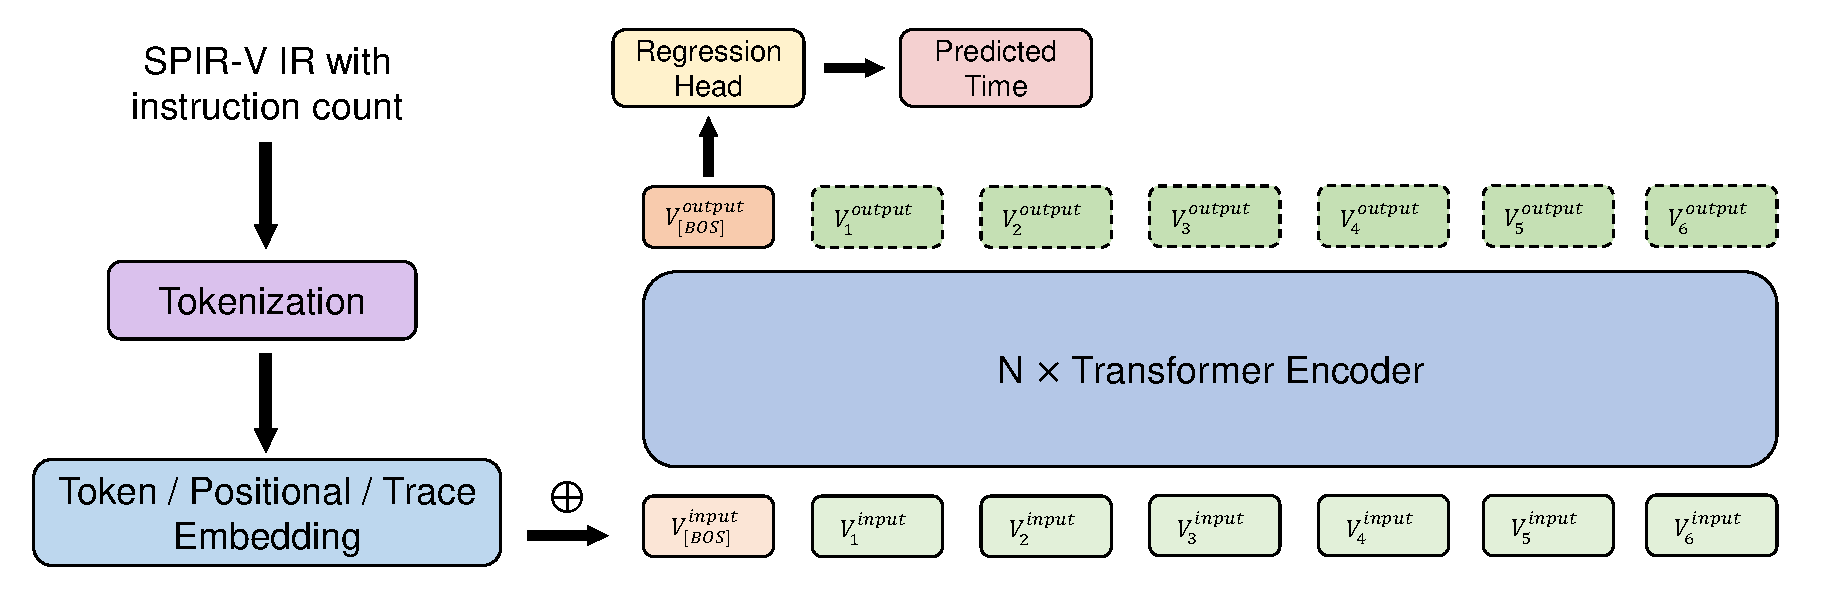
\includegraphics[width=1\linewidth]{figures/ShaderPerFormer(1)_20240103233446.pdf}
  \caption{ShaderPerFormer 模型概览}
  \label{fig:spf_overview}
\end{figure}

\label{sec:model}

%%%% FIX ME BEGIN HERE %%%%

第 \ref{sec:pl_understanding} 节提到,程序语言理解领域中广泛应用了基于 Transformer 的模型。类似的,本研究中的预测器采用类似 BERT\cite{devlin-etal-2019-bert} 架构的 Transformer 来构建回归预测模型。我们将这个基于神经网络的着色器程序性能模型命名为 ShaderPerFormer。

具体来说,图 \ref{fig:spf_overview} 给出了 ShaderPerFormer 的模型概览。我们首先将带有指令跟踪信息的 SPIR-V 交给 SPIR-V 分词器(tokenizer)进行分词。分词后,我们根据每个词元(token)、其所在的位置和其对应的指令的指令追踪得到的运行计数生成该词元对应的嵌入,从而作为 N 层Transformer编码器的输入。经过 N 层 Transformer 编码器的运算后,我们从最后一个Transformer编码器的输出中提取第一个词元对应的特征向量(latent vector),将其输入到回归头(regression head),并获得预测的时间。

\subsection{SPIR-V 分词器}

同第 \ref{sec:language_model} 节中的介绍一致,语言模型通常需要分词器来将输入的语言内容转换为词元序列。这其中,自然语言处理模型多使用在语料上自学习的分词器,如 BPE \cite{sennrich-etal-2016-neural}、SentencePiece \cite{kudo-richardson-2018-sentencepiece} 等。然而,由于本预测器处理的输入为 SPIR-V IR 构成的程序语言,而 SPIR-V IR 有规范定义的指令和操作数类型及其格式,故而我们认为一个专门设计的分词方案将会比基于学习的分词方案更加高效、易于编写和校验,且可以规避由于部分操作符出现次数的稀疏性给分词算法带来的问题。

算法 \ref{alg:tokenizer} 展示了我们提出的 SPIR-V 分词器的主要算法。其中,TokenizeModule 函数在输出一个 \verb|[BOS]| 词元后,会获得该 SPIR-V 模块的入口函数和其引用的所有函数,并且将其顺序排列;之后,对于每个函数中的每条指令,TokenizeInst 会将其进行分词,并利用 PushToken 函数顺序输出词元。对于字符串、整数和浮点数字面值,分词器统一采用转换为字符串、增加 offset 进行原样输出的方法进行分词。

这里的分词器在操作 SPIR-V 的部分同样使用了 SPIRV-Tools 提供的 SPIR-V 操作和变换的基础设施。类似第 \ref{sec:perf_measure} 节中的做法,我们在此处同样使用 pybind11 来将上述过程中涉及 C++ 的部分封装为 Python 扩展,以方便在 Python 中进行调用。

\begin{algorithm}
    % \SetAlgoLined %显示end
	\caption{SPIR-V 分词例程伪代码}%算法名字
    \label{alg:tokenizer}
\SetKwFunction{FTokenizeInst}{TokenizeInst}
\SetKwFunction{FTokenizeModule}{TokenizeModule}
\SetKwFunction{FTokenizeStringLiteral}{TokenizeStringLiteral}
\SetKwFunction{FPushToken}{PushToken}
\SetKwProg{Fn}{Function}{:}{}


\Fn{\FTokenizeStringLiteral{str}}{
    \ForEach{ch $\in$ str}{
        \tcc{PushToken($tok$) 用来输出一个词元 $tok$}
        \FPushToken{SymbolOffsets::ByteEncodedLiteralBegin + ch};
    }
}

\Fn{\FTokenizeInst{spirv\_inst}}{
    \FPushToken{SymbolOffsets::OpCodeBegin + spirv\_inst.opcode()}

    \ForEach{operand $\in$ spirv\_inst}{
        \uIf{isIdType(operand)}{
            \FPushToken{SymbolOffsets::IdBegin + operand.AsId()}\;
        }
        \uElseIf{isStringLiteral(operand)}{
            \FTokenizeStringLiteral{operand.AsString()}\;
        }
        \uElseIf{isIntegerLiteral(operand) or isFPLiteral(operand)}{
            \FTokenizeStringLiteral{to\_string(operand.AsNum())}\;
        }
    }
}

\Fn{\FTokenizeModule{spirv\_module}}{
    \tcc{首先输出一个 [BOS] 词元,[BOS] 词元在特殊符号中编号为 1}
    \FPushToken{SymbolOffsets::SpecialSymbolBegin + 1}\;
    \tcc{获得入口函数及其引用的所有函数的列表}
    funcs \gets spirv\_module.collectCallTreeFromRoots()\;
    \ForEach{f $\in$ funcs}{
        \ForEach{inst $\in$ f}{
            \FTokenizeInst{inst};
        }
    }
}


\end{algorithm}

% 本方法使用的分词器是用 C++ 编写的,并同性能测试例程一起作为 Python 扩展存在。它解析SPIR-V,并按函数进行分词。我们从入口点函数开始分词,然后以深度优先的顺序对从入口点函数可达的所有函数进行分词。我们在函数内部逐条指令进行分词。此外,在分词程序的开始处还单独添加了一个 \verb|[BOS]| 词元。

% 在SPIR-V指令中,操作码和ID操作数是32位整数,我们将它们一对一映射到词元。对于一些可以跨越任意字节数的字面量操作数,我们将每个字节一对一映射到词元。

% \subsection{指令计数上下文嵌入}
\subsection{指令词嵌入生成}

\begin{figure}[h]
  \centering
  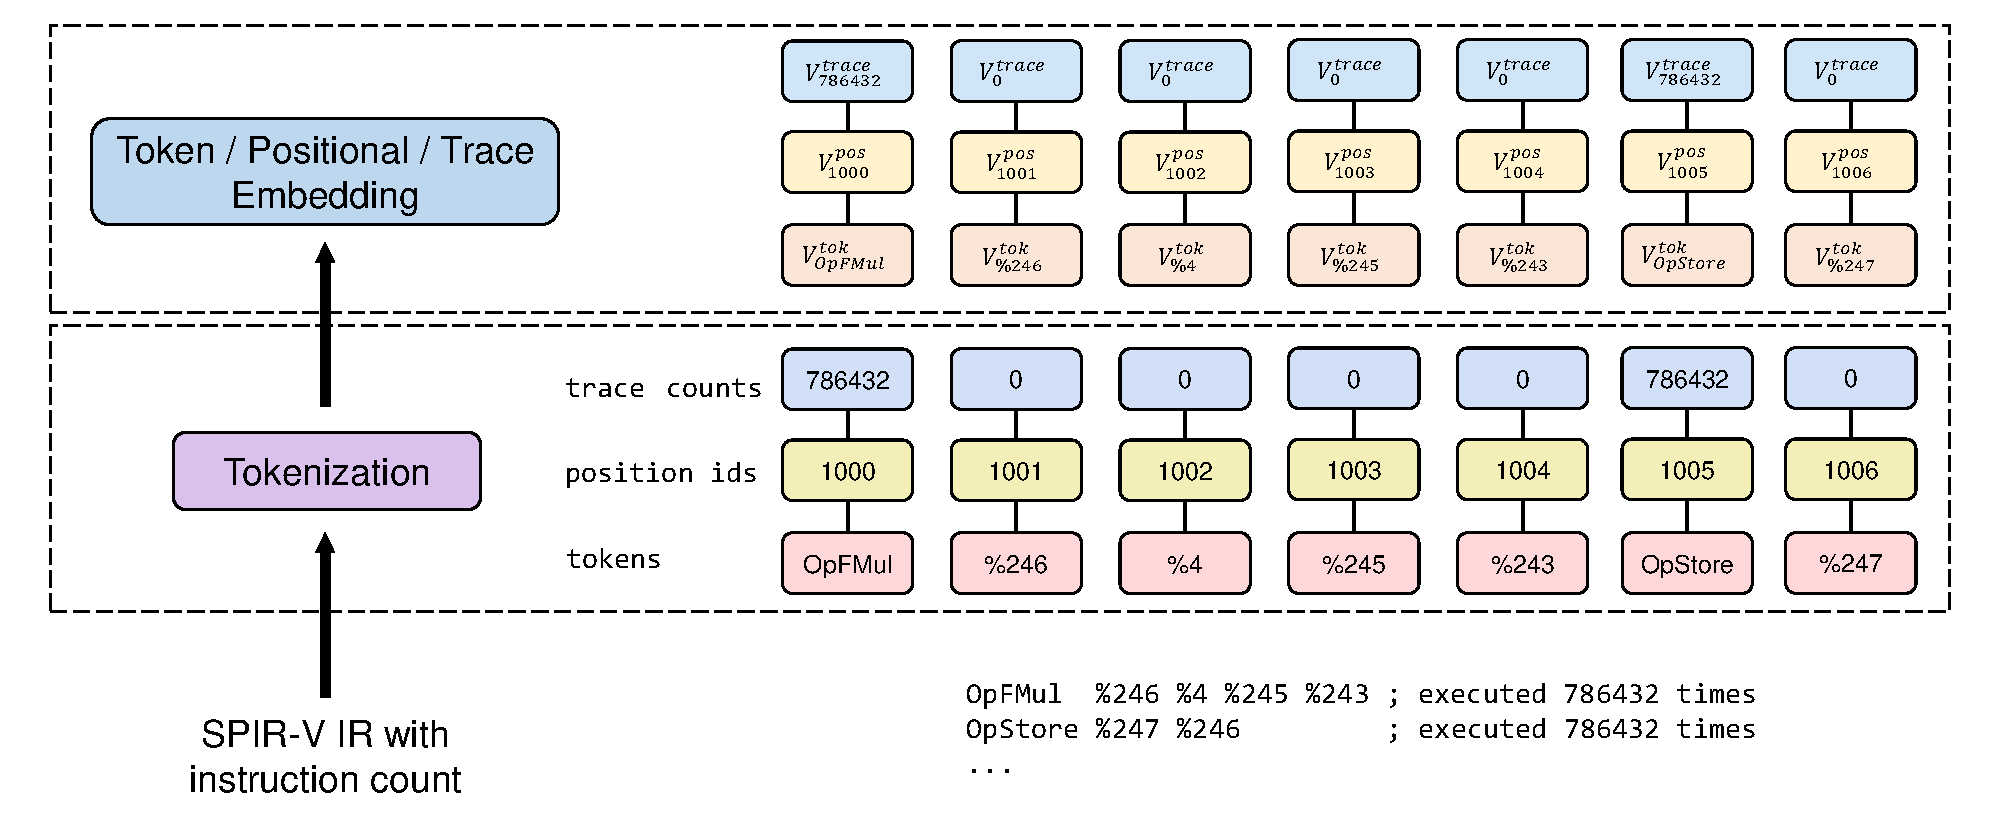
\includegraphics[width=1\linewidth]{figures/tokandembed.pdf}
  \caption{ShaderPerFormer 的分词和词嵌入向量生成过程}
  % \note{注:为了可读性,分词后的操作码 (opcode) 和操作数 (operand) 词元以文本形式表示。本图展示了从位置 1000 开始的一小段中间表示指令序列,其中的指令被执行了 786432 次,正好是 1024 $\times$ 768 屏幕分辨率下每片元执行一次的中间表示指令。因篇幅所限,OpStore 指令的操作数分词结果在此没有画出。}
  \label{fig:spf_embedding}
\end{figure}

图 \ref{fig:spf_embedding} 展示了 ShaderPerFormer 的分词和词嵌入向量生成过程。为了可读性,分词后的操作码 (opcode) 和操作数 (operand) 词元以文本形式表示。该图展示了从位置 1000 开始的一小段中间表示指令序列,其中的指令被执行了 786432 次,正好是 1024 $\times$ 768 屏幕分辨率下每片元执行一次的中间表示指令。因篇幅所限,OpStore 指令的操作数分词结果在此没有画出。

从图 \ref{fig:spf_embedding} 中可以看到,ShaderPerFormer 第 $ i $ 个位置的词嵌入向量 $ \mathbf{V}^{\text{input}}_i $ 分为三个部分的组合:
\begin{equation}
\mathbf{V}^{\text{input}}_i = \mathbf{V}^\text{tok}_{t_i} +\mathbf{V}^\text{pos}_i + \mathbf{V}^\text{trace}_{m_i},
\end{equation}
其中 $t_i$ 和 $m_i$ 分别是位置 $i$ 的词元和词元对应的指令的运行计数。

$ \mathbf{V}^\text{tok}_{t_i} $ 为位置 $i$ 的词元本身的嵌入,而 $\mathbf{V}^\text{pos}_i$ 为绝对位置 $ i $ 的嵌入。和 BERT 的做法相符,这两个嵌入均采用一对一映射的可学习嵌入(learnable embedding)。

$ \mathbf{V}^\text{trace}_{m_i} $ 为位置 $i$ 的词元对应的指令的运行计数的嵌入。然而,由于指令运行计数以 64 位整数表示,且实测因其用 32 为整数表示时会发生溢出现象,故而其至少横跨 0 到 $2^{31} - 1$ 的区间。如此一来,采用一对一映射的可学习嵌入来生成指令运行计数嵌入是不可行的。

与 \citet{Born2023} 中的数值编码方案类似,我们选择直接将待编码的指令计数转换为二进制形式作为嵌入向量,并用 0 填充额外的维度。给定 $\overline{x_i}$ 表示 $x$ 的二进制表示中的第 $i$ 位数字,跟踪嵌入 $\mathbf{V}^{\text{trace}}_x$ 可以写成
\begin{equation}
\mathbf{V}^{\text{trace}}_x = [\overline{x_0}, \overline{x_1}, \dots, \overline{x_{63}}, 0, \dots, 0].
\end{equation}
这样,就解决了指令计数的嵌入生成问题。

值得注意的是,$ \mathbf{V}^\text{trace}_{m_i} $,即位置 $i$ 的词元对应的指令的运行计数,只会在该指令对应的第一个词元处可能被设置为非 0 的值。在 SPIR-V 中,一个指令经常有多个操作数,而其每个操作数根据算法 \ref{alg:tokenizer} 又可能对应多个词元。在所有这些词元的指令计数嵌入中,只有第一个词元的指令计数嵌入 $ \mathbf{V}^{\text{trace}} $ 会可能被设置为非零向量。

\subsection{编码器和输出层}

\label{sec:encoder_and_output_layer}

ShaderPerformer 使用 9 层的 Transformer 编码器,隐藏层维度为 768,注意力头数为 12。在最后一层的 Transformer 编码器后进入输出层。输出层会选取第一个词元(固定为 \verb|[BOS]|)对应的特征向量,并将其送入回归头进行输出预测。

选择固定的 \verb|[BOS]| 词元对应的特征向量的主要原因是为了增强模型的稳定性。Transformer 模型的每一层都会在所有词元位置处计算注意力,而一个稳定的固定词元作为输出可以降低不稳定的后续输入对输出带来的影响。此种做法在 BERT \cite{devlin-etal-2019-bert}中也得到了应用。

回归头和 Transformer 编码器一样,同样应用了一些 Dropout 以减少过拟合的风险。回归头的计算方式如下:
\begin{equation}
    \label{eq:reg_head}
    \text{RegressionHead}(x) = \text{Linear}(\text{Dropout}(\text{Tanh}(\text{Linear}(\text{Dropout}(x))))).
\end{equation}

同时,由于 ShaderPerFormer 需要将整个着色器程序的 SPIR-V 作为模型的输入,这样一来,模型可以接受的序列长度将直接影响其训练和使用时的泛用性。针对于 Transformer 训练时内存占用较高的问题,我们在 Transformer 的编码器中的注意力部分使用了低内存占用的 Memory Efficient Attention \cite{rabe2022selfattention} 注意力实现。

\subsection{归一化方式和损失函数}

由于我们的性能样本时间跨度从 $10^{-6}$ 秒到 $10^{-1}$ 秒不等,如果在没有归一化的情况下直接使用小批量梯度下降法(mini-batch gradient descent)来优化均方误差(MSE),可能会导致损失函数不稳定。因此,我们选择对我们的数据输入进行对数归一化,即对数据集中的每一个时间 $t$ 都进行 $\log(t)$ 变换。

我们使用均方误差(MSE)作为 ShaderPerFormer 的损失函数。考虑到我们使用的归一化方法,损失函数也可以被称为均方对数误差(Mean Squared Logarithmic Error,MSLE)。

在对数尺度上,数据的变化更加平滑,这有助于模型更好地学习数据的分布。同时,MSLE损失函数鼓励模型对预测值和真实值的对数进行准确的估计,从而在指数变换回原始尺度后,能够获得较为准确的预测结果。

\section{实验和分析}

\subsection{基线方法}

\citet{10.1145/2816795.2818104} 使用了下面的启发式来估计着色器在一个绘制流水线阶段的性能,
\begin{align}
t &= N_\text{scalarOps} + 100 \times N_\text{textureOps},
\end{align}
其中 $N_\text{scalarOps}$ 是着色器程序中标量操作的数目, $N_\text{textureOps}$ 是着色器程序中纹理采样操作的数目。这里的常数 $100$ 是一个原方法中随意设置的值,用于表示标量操作和浮点操作之间性能的相对关系。

将这个思路进行简单的推广后,我们使用两种方法来作为基线,
\begin{align}
\label{eq:sh} t &= c_\text{inst} \cdot N_\text{inst} \\
\label{eq:pilr} t &= \sum_{i=1}^{M} c_{\text{inst}_{i}} \cdot N_{\text{inst}_{i}}.
\end{align}

\begin{enumerate}
    \item 简单启发式(Simple Heuristics,SH): 如式 (\ref{eq:sh}),我们为 IR 中的每条指令都赋予一个统一的指令时间开销 $c_{inst}$,并且乘以着色器运行时执行总 IR 指令数 $N_{inst}$,以得到预测的着色器运行总时间。
    \item 逐指令线性回归(Per Instruction Linear Regression,PILR): 如式 (\ref{eq:pilr}) 所示,我们为 IR 中的每种指令赋予一个统一的时间开销 $c_{inst_i}$,并且乘以该种指令运行时执行的总次数 $N_{inst_i}$,并对每个指令种类求和,以得到预测的着色器运行总时间。
\end{enumerate}

% TODO: introduce regression code

\subsection{性能数据集分析}

我们通过将 iTime 和 iFrame 设置为 1 来固定着色器的 Uniform 输入值,并使用第 \ref{sec:dataset} 节中描述的方法在 5 种不同的GPU平台上收集了我们的数据集。这些平台涵盖了多种不同的架构、厂商和 GPU 形态,包括桌面端和移动端显卡、独立和集成显卡。详细的环境信息可以参见表 \ref{table:envInfo}。

\begin{table}[h]
    \centering
    \caption{测试的 GPU 平台的全名和类型一览}
    \label{table:envInfo}
    \begin{tabular}{llll}
    \toprule
        \textbf{缩写} & \textbf{全名} & \textbf{厂商} & \textbf{类型} \\ 
    \midrule
        RTX3060 & NVIDIA GeForce RTX 3060 & NVIDIA & 桌面端独立显卡 \\ 
        UHD630 & Intel UHD Graphics 630 (CML GT2) & Intel & 桌面端集成显卡 \\ 
        RTX4060 & NVIDIA GeForce RTX 4060 Laptop GPU & NVIDIA & 移动端独立显卡 \\ 
        GTX1660Ti & NVIDIA GeForce GTX 1660 Ti & NVIDIA & 移动端独立显卡 \\ 
        RX7900GRE & AMD Radeon RX 7900 GRE & AMD & 桌面端独立显卡 \\ 
    \bottomrule
    \end{tabular}
\end{table}

在数据集的构建过程中,本研究过滤掉了使用预测器尚未支持特性的着色器样本,以及那些可能存在错误的样本。由于着色器语言中的未定义行为在驱动程序之间往往存在微妙的实现差异,且不同平台有不同的 GPU 上下文超时时间设置,因此作为有效性能样本保留的数量在我们测试的不同平台上略有不同。表 \ref{table:datasetFilters} 给出了不同平台上性能样本经过滤后的数量一览。图 \ref{fig:instStat} 给出了测试平台之一的 RTX3060 平台中,IR 层次上有效性能样本特征的统计分布。其中,图 \ref{fig:instStat}(a) 给出了着色器指令按 SPIR-V 规范进行类别分解后的指令类别占比,而图 \ref{fig:instStat}(b) 给出了通过过滤器的性能样本的着色器指令数分布。 

\begin{figure}[h]
  \centering
      \centering
      \subfloat[着色器指令类别分解]{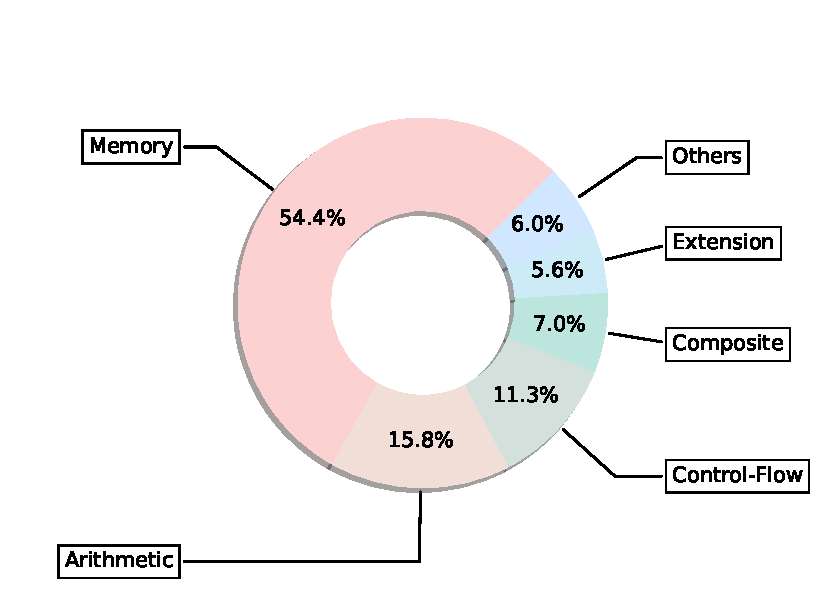
\includegraphics[width=.45\textwidth]{figures/opcode_distribution.pdf}}
      \qquad
      \subfloat[着色器指令数分布]{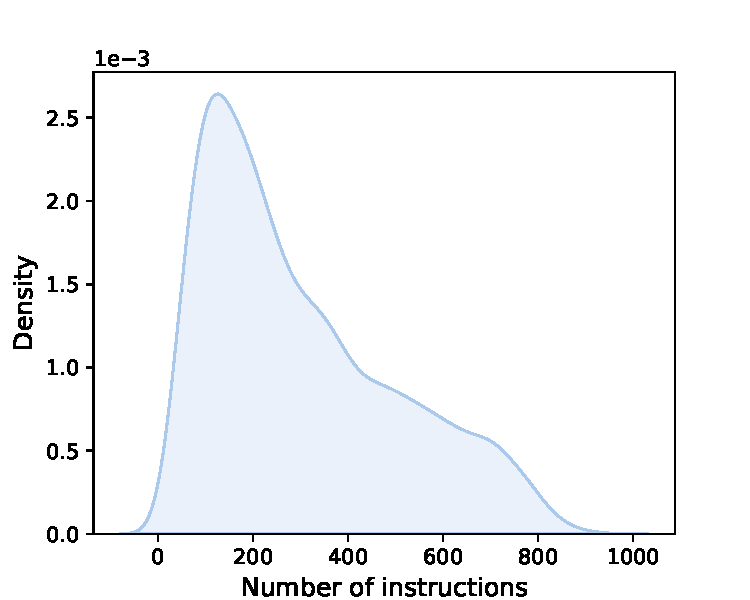
\includegraphics[width=.45\textwidth]{figures/opcode_count_snapshot.pdf}}
  % \caption{RTX3060 平台上通过所有过滤器的着色器性能样本分析。SPIR-V 指令的类型来源于 SPIR-V 规范。}
  \caption{RTX3060 平台上通过所有过滤器的着色器性能样本分析}
  \label{fig:instStat}
\end{figure}

\begin{table}[h]
    \centering
    \caption{在各个过滤阶段过后剩余的着色器性能样本数量一览}
    \label{table:datasetFilters}
    % \resizebox{\columnwidth}{!}{
    \begin{tabular}{l|ccccc}
    \toprule
        \textbf{过滤器}  & RTX3060 & RX7900GRE & UHD630 & RTX4060 & GTX1660Ti \\
    \midrule
        Shadertoy 着色器        & \multicolumn{5}{c}{27911} \\ 
        单渲染通道着色器        & \multicolumn{5}{c}{20669} \\ 
        运行成功           & 13871  & 14084  & 13856 & 14094 & 13913 \\ 
        追踪成功         & 13870  & 14080  & 13850 & 14090 & 13913 \\ 
        非纯黑纯白       & 13376  & 13925  & 13364 & 13484 & 13379 \\ 
        在词元长度限制内 & 10794  & 11360  & 10784 & 10935 & 10806 \\ 
        在时间限制内         & 10794  & 11360  & 10781 & 10935 & 10797 \\
    \bottomrule
    \end{tabular}
    \note{注:\textit{非纯黑纯白}和\textit{在时间限制内}用来过滤可能有 bug 的着色器。 \textit{在词元长度限制内} 用来过滤对于 ShaderPerFormer 来说过长的着色器。}
    % }
\end{table}

\begin{figure}[h]
  \centering
  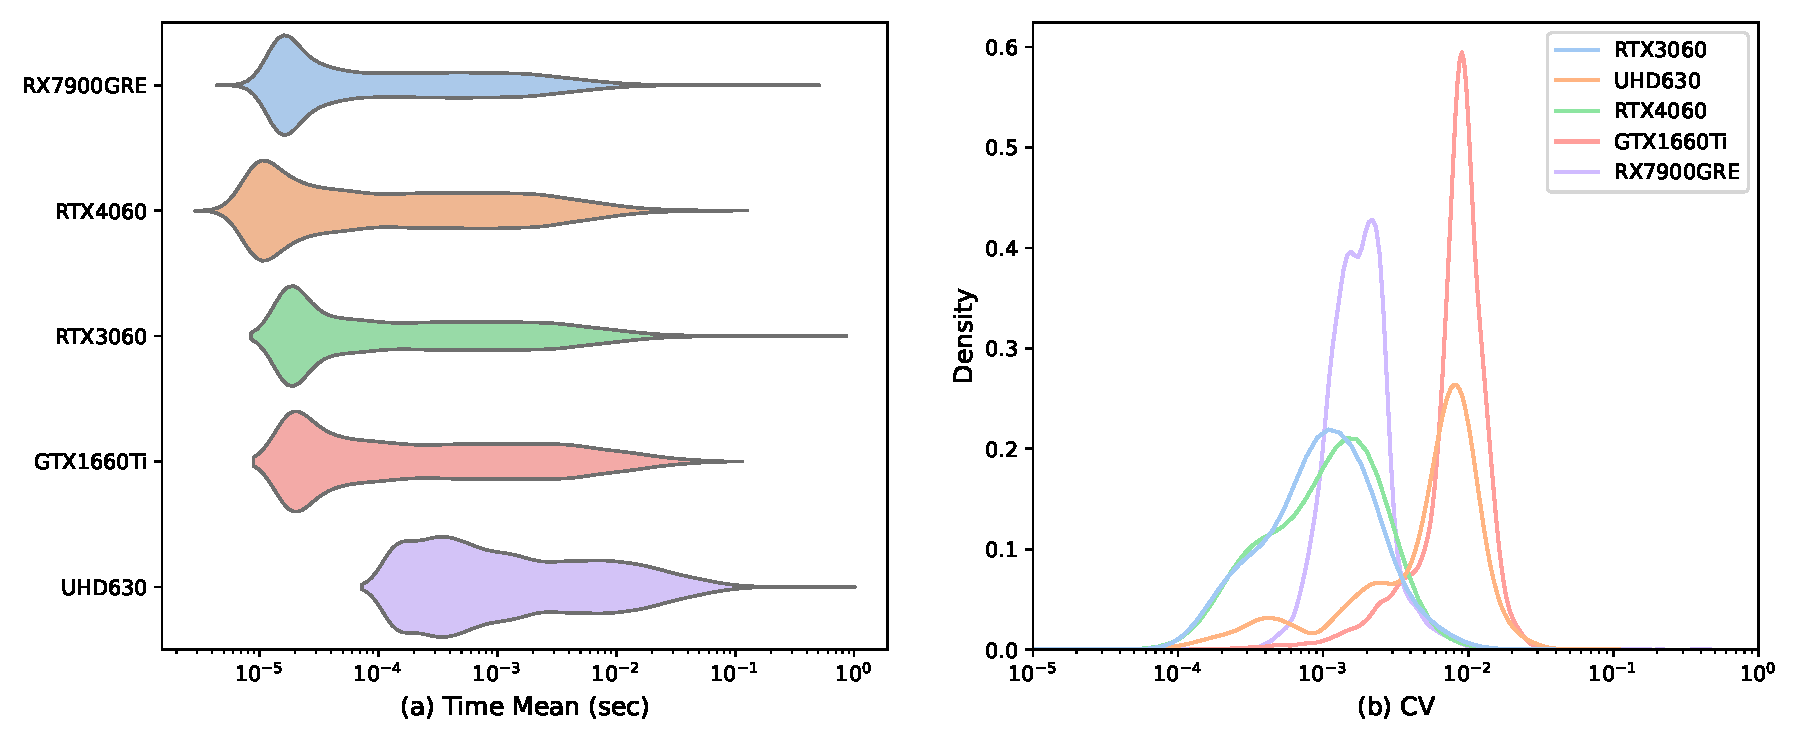
\includegraphics[width=1.0\linewidth]{figures/time_mean_and_cv.pdf}
  \caption{(a) 各 GPU 平台上性能样本关于时间的分布 (b) 各 GPU 平台测得的变异系数分布}
  \label{fig:archTimeMeanCV}
\end{figure}

从收集到的性能样本中可以观察到,不同平台上着色器的性能关系是并非简单的线性关系所能刻画的。图 \ref{fig:archTimeMeanCV}(a) 展示了各个不同 GPU 平台上,性能样本相对于其运行时间的小提琴分布图。从分布图中可以得出,平台间的分布形状都有或多或少的差异,而这种差异在 UHD630 平台上尤其显著。在 UHD630 平台上,由分布整体靠右可以得到,该平台平均性能较其它平台更低,且由分布形状可知其性能样本的分布特点也与其它 GPU 平台显著不同。故而从一般意义上来说,使用其它平台上的着色器执行时间的进行简单的按比例线性缩放,来估计某个平台上的时间是存在困难的。

在收集性能样本时,算法 \ref{alg:profile} 中设计了相应的重复测量环节,以确保收集到的数据足够精确。经过探索,本研究在数据集收集过程中,其算法中的 {num\_cycles} 和 {num\_trials} 分别取 30 和 10。我们还额外检查了每个着色器的 10 次测量的计算出的变异系数(Coefficient of Variation,CV),以确保我们收集的性能数据具有足够的精度。变异系数 $ \symup{CV} $ 的定义为
$$
\symup{CV} = \frac{\sigma}{\mu},
$$
即测量值构成的序列的标准偏差与其平均值的比率,其能够比较有效的刻画我们收集到的性能样本的相对精度。

图 \ref{fig:archTimeMeanCV}(b) 提供了所有测量平台的变异系数,从中可以得出结论,本研究测量的大多数平台的变异系数小于$3\%$。我们认为该变异系数的上界所对应的精度,可以满足对于后续的使用和分析的需要。

\subsection{性能模型预测分析}

\subsubsection{数据集划分与训练}

\label{sec:training}

图 \ref{table:datasetFilters} 给出了经过过滤各个架构中的着色器性能样本。每个性能样本都对应着一个着色器,而鉴于各个平台上被过滤后剩下的性能样本数量不一,如果将每个平台剩余的性能样本单独进行数据集划分的话,则可能因为在不同平台上不一致的划分影响后续评估的有效性。故而,我们首先将不同平台剩余的性能样本对应的着色器取并集,在这个并集中将性能样本随机划分为训练集、测试集和验证集,且比例为训练集:测试集:验证集=$80:5:15$。

ShaderPerFormer 的训练使用一块 24 GB 显存的 NVIDIA GeForce RTX 4090 完成。得益于 xformers \cite{xFormers2022}库中 Memory Efficient Attention 的注意力算子实现\cite{rabe2022selfattention},ShaderPerFormer 的模型可以在第 \ref{sec:encoder_and_output_layer} 节提及的模型配置下使用 4096 的最大序列长度进行训练。在上述模型配置下,我们使用 2 的批次大小(batchsize),并通过 20 步的梯度累积(gradient accumulation)来得到 40 的等效批次大小。

我们使用 Adam \cite{Kingma2014AdamAM} 作为优化器,学习率设为 $3 \times 10^{-5}$,使用默认的 Adam 配置($\beta_1=0.9, \beta_2=0.999, \epsilon=1 \times 10^{-8}$),并使用预热比例(warmup ratio)为 0.1 的线性学习率预热。每种架构上的模型均训练 50 个迭代轮次(epoch),并挑选出在轮次结束时,在测试集上具有最佳 MAPE (Mean Average Percentage Error, 平均绝对百分比误差)的模型权重作为最优模型权重,并作为后续评估用的模型。

\subsubsection{基线比较}

我们在收集的 5 个平台上分别评估了两种基线方法和用 \ref{sec:training} 中的训练配置训练出的 ShaderPerFormer 预测模型的性能,并在划分出的验证集上报告预测时间与实际测量时间之间的 MAPE。评估的结果参见表 \ref{table:mainResults}。

从表中可以看出,ShaderPerFormer 在所有测试方法中是最准确的。与简单启发式方法和逐指令线性回归这两种基线方法相比,本研究提出的 ShaderPerFormer 方法在 5 个待测平台上的平均 MAPE 分别提高了 25.25\% 和 8.26\%,并达到了 35.96\% 的平均 MAPE。

对于着色器优化任务来说,在进行优化变体评估时通常只需要确定给定的变体之间的性能的相对排序,而不需要其绝对值。这种情形下的准确度可以用 Spearman 相关系数来进行刻画。Spearman 相关系数可以刻画两个统计变量之间的秩的相关性,且当两组统计观测值之间由相似的秩时相关系数较高。两组组在秩的意义下完美单调增加的序列的 Spearman 相关系数为 1。表 \ref{table:mainResults} 还报告了每种方法的预测结果与测量结果之间的 Spearman 相关系数。与其它基线方法相比,ShaderPerFormer 在所有测试平台上都拥有最高的 Spearman 相关系数。

MAPE 和 Spearman 系数缺乏对于不同运行时间分组的着色器性能样本,其预测精度的刻画能力。如图 \ref{fig:archHeatmap} 所示,为了让三种预测模型的结果得到更直观的展示,我们给出了在各个平台上,基线模型和 ShaderPerFormer 方法的预测和实际结果的分布热力图。该热力图的横轴为测量得到的 10 次真实时间的均值,纵轴为性能预测模型预测的时间。热力图的中央部分被切分为 50 $\times$ 50 的格子,每个格子中用颜色表示该区域中分布的样本数量。可以看出,ShaderPerFormer 模型较其它两个模型,在较高性能和较低时间的性能样本部分都拥有不错的表现,且接近 $y=x$ 的直线。

\begin{figure}[htbp]
  \centering
  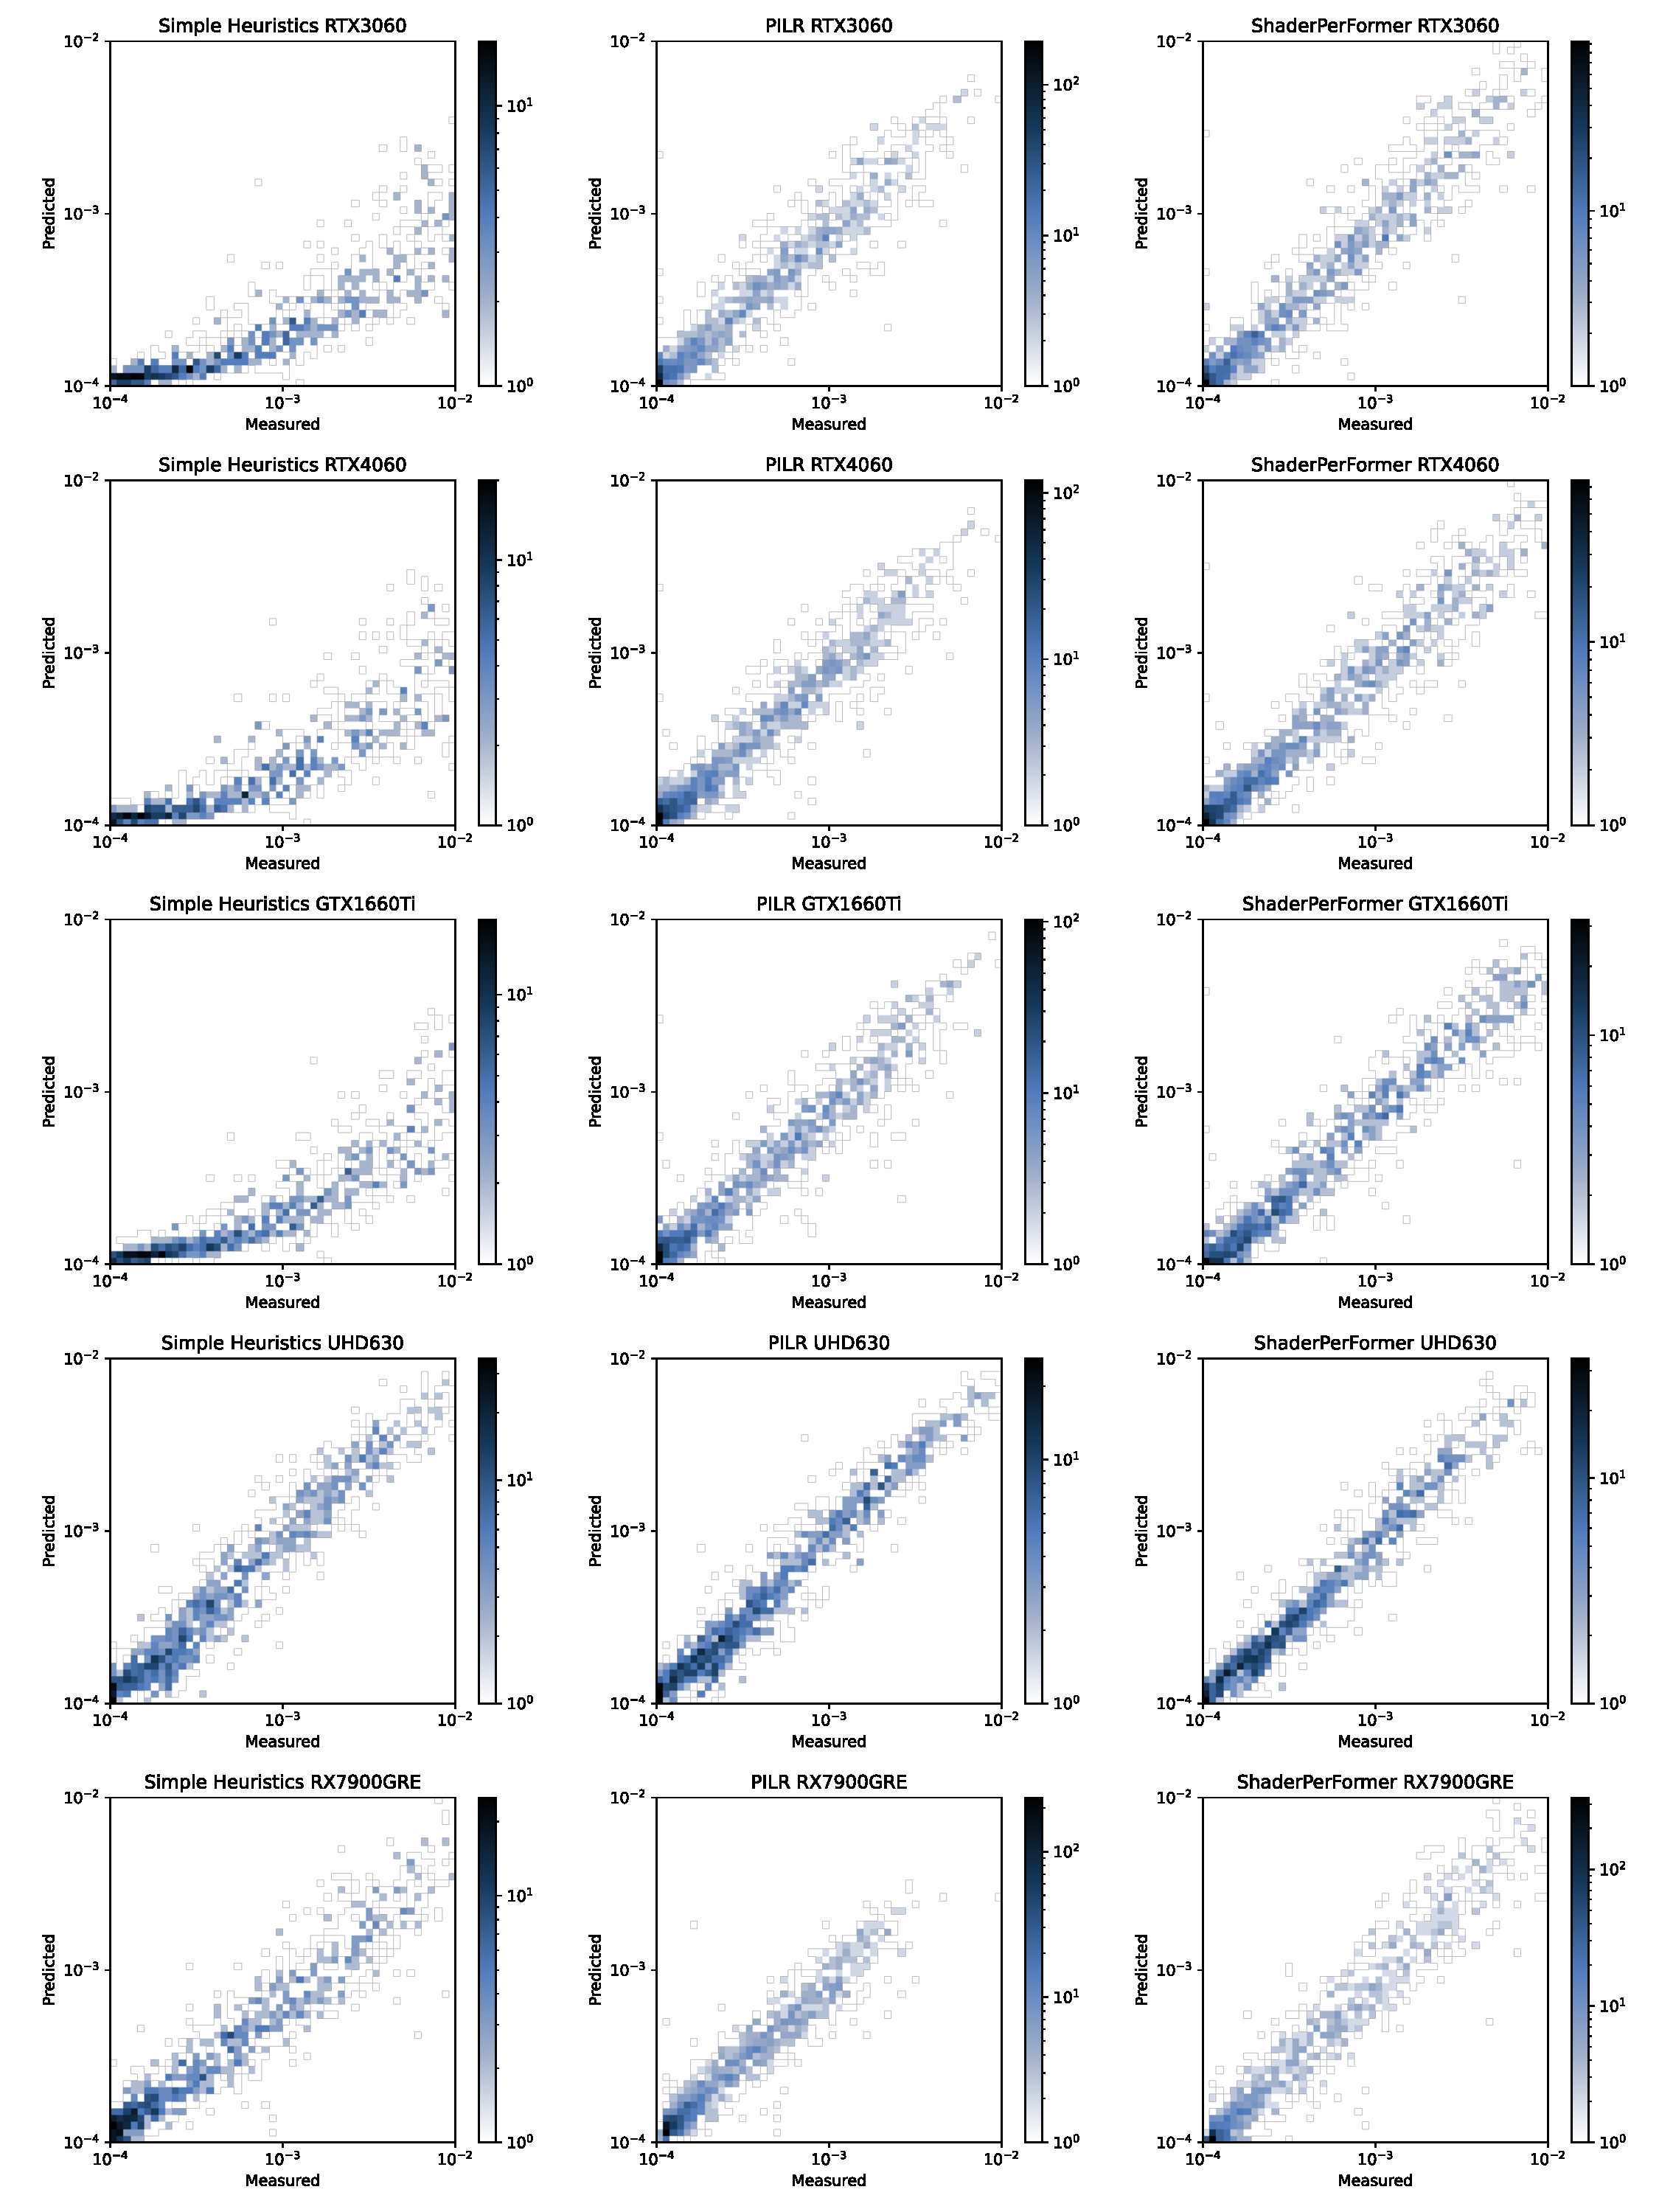
\includegraphics[width=1.0\linewidth]{figures/archHeatmapRefined.pdf}
  \caption{各个平台上,基线模型和本文方法的预测和实际结果的分布热力图}
  \note{注:SH 代表简单启发式,PILR 代表逐指令线性回归,ShaderPerFormer 代表本研究提出的基于神经网络的着色器性能预测方法。}
  \label{fig:archHeatmap}
\end{figure}

这些评估结果表明,ShaderPerFormer 在预测着色器性能方面相比于基线方法具有一定比较优势,特别是在需要对多个着色器进行性能排序的场景中。Spearman 相关系数的高值表明,ShaderPerFormer 能够更有效地识别出着色器性能排序,这对于开发者进行着色器性能优化有一定价值。此外,ShaderPerFormer 在需要精确性能评估的场合,较现有的着色器性能评估工作也更具有竞争力。

\begin{table}[h]
    \centering
    \caption{各 GPU 平台上的验证集下的模型性能结果}
    \label{table:mainResults}
    \begin{tabular}{l|cccccc}
    \toprule
    % \multicolumn{3}{c}{\textbf{MAPE}}
    % \multirow{2}{*}{\textbf{Platform}}
        ~  & \multicolumn{2}{c}{SH} & \multicolumn{2}{c}{PILR} & \multicolumn{2}{c}{ShaderPerFormer (\textbf{Ours})} \\ 
        \textbf{平台}          & MAPE & Spearman & MAPE & Spearman & MAPE & Spearman \\
    \midrule
        RTX3060 &  75.26\% & 0.9584 &  46.90\% & 0.9200 & \textbf{40.44\%} & \textbf{0.9642} \\
        UHD630 &  30.73\% & 0.9594 &  27.32\% & 0.9676 & \textbf{26.60\%} & \textbf{0.9722} \\
        RTX4060 &  81.17\% & 0.9588 &  55.60\% & 0.9290 & \textbf{44.62\%} & \textbf{0.9632} \\
        GTX1660Ti &  82.56\% & 0.9607 &  54.99\% & 0.9353 & \textbf{41.59\%} & \textbf{0.9681} \\
        RX7900GRE &  36.32\% & 0.9510 &  36.28\% & 0.9433 & \textbf{26.54\%} & \textbf{0.9578} \\
    \midrule
        平均 & 61.21\% & --- & 44.22\% & --- & \textbf{35.96\%} & --- \\
    \bottomrule
    \end{tabular}
    \note{注:SH 代表简单启发式,PILR 代表逐指令线性回归,ShaderPerFormer 代表本研究提出的基于神经网络的着色器性能预测方法。最佳的性能指标以加粗字体展示。}
\end{table}

\subsection{指令追踪信息对预测的影响}

为了证明我们提出的指令跟踪计数信息对着色器性能预测任务的重要性,本节进行消融实验,即比较在没有指令追踪信息的的情况下,ShaderPerFormer 方法和基线方法的性能。

为了确保公平比较,在消融实验中我们保持 ShaderPerFormer 的网络架构不变,并将所有位置的指令计数设置为 1。这意味着所有位置的指令跟踪嵌入均变为了 $\mathbf{V}^\text{trace}_{1} = [1, 0, \dots, 0]$,从而消除了指令的追踪信息产生的计数的嵌入对网络的影响。

对于简单启发式和逐指令线性回归两种基线方法,我们进行如下的更改:
\begin{enumerate}
    \item 简单启发式:我们将式 (\ref{eq:sh}) 中的 $N_{inst}$ 由着色器\textbf{运行时}执行的总 IR 指令数替换为着色器程序总 IR 指令数。
    \item 逐指令线性回归:我们将式 (\ref{eq:pilr}) 中的 $N_{inst_i}$ 由着色器\textbf{运行时}执行的该种指令数目替换为着色器该种指令数目。 
\end{enumerate}

对于基线方法的修改相当于,在两种基线方法训练时,假设着色器中的每条指令“执行”一次且仅“执行”一次,其余细节保持不变。

如表 \ref{table:ablationTrace} 所示,指令跟踪被证明对于 ShaderPerFormer 和逐指令线性回归方法起到了在 MAPE 和 Spearman 相关系数意义上、对不同待测 GPU 平台一致的效果改善,在简单启发式模型中,部分平台的 MAPE 测量结果得到了效果改善,而所有平台的 Spearman 相关系数都得到了改善。

这一结果证明了指令跟踪计数信息对着色器性能预测任务的重要性。通过考虑指令的实际执行次数,我们的方法能够更准确地捕捉到着色器执行时间的复杂性。这种改进对于ShaderPerFormer 和 PILR 这样模型尤其重要,因为它们依赖于输入数据的质量和代表性来做出准确的预测。简单启发式方法虽然在某些平台上表现出了改进,但可能不如前两者那样一致或显著,这也表明更复杂的模型可以更好地利用跟踪计数信息。

\begin{table}[h]
    \centering
    \caption{在 ShaderPerFormer 和两种基线方法上进行的指令追踪信息的消融实验结果}
    \label{table:ablationTrace}
    \begin{tabular}{l|l|cccc}
    \toprule
        \multirow{2}{*}{\textbf{方法}} & \multirow{2}{*}{\textbf{平台}} & \multicolumn{2}{c}{\textbf{MAPE}} & \multicolumn{2}{c}{\textbf{Spearman}} \\ 
        ~                                & ~                                  & 无追踪信息 & 有追踪信息 & 无追踪信息 & 有追踪信息 \\ 
    \midrule
        \multirow{5}{*}{SH}   & RTX3060             & 76.02\%  & \textbf{75.26\%} &  0.7131 &  \textbf{0.9584} \\
        ~ & UHD630                                  & 66.97\%  & \textbf{30.73\%} &  0.7152 &  \textbf{0.9594} \\
        ~ & RTX4060                                 & \textbf{79.54\%}  & 81.17\% &  0.7118 &  \textbf{0.9588} \\
        ~ & GTX1660Ti                               & \textbf{80.20\%}  & 82.56\% &  0.7142 &  \textbf{0.9607} \\
        ~ & RX7900GRE                               & 68.65\%  & \textbf{36.32\%} &  0.6857 &  \textbf{0.9510} \\ \hline
        \multirow{5}{*}{PILR} & RTX3060             & 86.43\%  & \textbf{46.90\%} &  0.8551 &  \textbf{0.9200} \\
        ~ & UHD630                                  & 72.87\%  & \textbf{27.32\%} &  0.8503 &  \textbf{0.9676} \\
        ~ & RTX4060                                 & 90.39\%  & \textbf{55.60\%} &  0.8563 &  \textbf{0.9290} \\
        ~ & GTX1660Ti                               & 90.26\%  & \textbf{54.99\%} &  0.8571 &  \textbf{0.9353} \\
        ~ & RX7900GRE                               & 81.19\%  & \textbf{36.28\%} &  0.8388 &  \textbf{0.9433} \\ \hline
        \multirow{5}{*}{\makecell{ShaderPerFormer \\(\textbf{Ours})}} & RTX3060              & 81.02\%  & \textbf{40.44\%} &  0.8608 &  \textbf{0.9642} \\
        ~ & UHD630                                  & 70.42\%  & \textbf{26.60\%} &  0.8749 &  \textbf{0.9722} \\
        ~ & RTX4060                                 & 98.10\%  & \textbf{44.62\%} &  0.7518 &  \textbf{0.9632} \\
        ~ & GTX1660Ti                               & 109.60\% & \textbf{41.59\%} &  0.8784 &  \textbf{0.9681} \\
        ~ & RX7900GRE                               & 51.16\%  & \textbf{26.54\%} &  0.8448 &  \textbf{0.9578} \\
    \bottomrule
    \end{tabular}
    \note{注:SH 代表简单启发式,PILR 代表逐指令线性回归,ShaderPerFormer 代表本研究提出的基于神经网络的着色器性能预测方法。最佳的性能指标以加粗字体展示。}
\end{table}